\documentclass[11pt]{article}

\usepackage{graphics}
\usepackage{html}

%\usepackage{xr-hyper}
\usepackage{hyperref}
\usepackage[usenames, dvipsnames]{color}
\usepackage{colortbl}
%\usepackage{calc}

% Sans fonts
\usepackage{sfmath}
\renewcommand{\familydefault}{\sfdefault}

\markright{PHYS328 Notes}

\setlength{\textwidth} {6.5 true in}
\setlength{\textheight}{9 true in}
\setlength{\hoffset} {-0.75 true in}
\setlength{\voffset} {-0.75 true in}
\setlength{\parindent} {12 pt}
\pagestyle{myheadings}

\title{PHYS328W Notes} \author{L.A. Riley} \date{Fall 2021}

\begin{document}

\thispagestyle{empty}

\maketitle

\section{DC Circuits}

\subsection{Ohm's Law and Ohmic Devices}
\label{sec:ohm}

The potential difference $V$ between the terminals of an \textbf{Ohmic
device} is directly proportional to the current $I$ flowing through it,
\begin{equation}
  V=IR
\label{eq:Ohm}
\end{equation}
The constant of proportionality $R$ is called the \textbf{resistance}
of the device. Equation~\ref{eq:Ohm} is known as \textbf{Ohm's
  Law}.
\textbf{Non-ohmic} devices do not follow the linear voltage-current
relationship of Ohm's law. Examples include diodes, thermistors,
photoresistors, and light-bulb filaments.

Ohmic devices called \textbf{resistors} are ubiquitous in
electronic circuits. When current flows through a resistor, power is
dissipated in the form of heat and light. The power dissipated in a
resistor given by
\begin{equation}
  P_\mathrm{diss} = I^2 R = \frac{V^2}{R}
\end{equation}

\subsection{Resistors in Series and Parallel}
\label{sec:serpar}

\begin{figure}[ht]
  \htmlimage{align='center'}{}
  \begin{center}
    \includegraphics{seriesparallel.eps}
    \caption{A pair of resistors connected (a) in series and (b) in
      parallel.}
    \label{fig:seriesparallel}
  \end{center}
\end{figure}

A pair of resistors can be connected either in \textbf{series} or in
\textbf{parallel} as shown in Figure~\ref{fig:seriesparallel}.  Note
that two wires emerge from each pair. The \textbf{equivalent
  resistance} $R_\mathrm{eq}$ of a pair of resistors is the resistance
between these two wires. The equivalent resistance of two or more
resistors connected in series is given by
\begin{equation}
  R_{eq} = R_1 + R_2 + R_3 + \ldots
  \label{eq:Rseries}
\end{equation}
and that of two or more resistors connected in parallel is given by
\begin{equation}
  \frac{1}{R_{eq}} = \frac{1}{R_1} + \frac{1}{R_2} + \frac{1}{R_3} +
  \ldots
  \label{eq:Rparallel}
\end{equation}
The notation $R_1||R_2||R_3...$ is sometimes used for the equivalent
resistance of parallel resistors.

A pair of resistors connected in series as shown in panel (a) of
Figure~\ref{fig:seriesparallel} is a \textbf{voltage divider}. The two
resistors share the total potential difference $V$ across the
pair according to
\begin{eqnarray}
  \nonumber
  V_1 & = & \frac{R_1}{R_1 + R_2} V \\ 
  V_2 & = & \frac{R_2}{R_1 + R_2} V
  \label{eq:Vdiv}
\end{eqnarray}

A pair of resistors connected in parallel as shown in panel (b) of
Figure~\ref{fig:seriesparallel} is a \textbf{current divider}. The two
resistors share the total current $I$ flowing into the pair according
to
\begin{eqnarray}
  \nonumber I_1 & = & \frac{R_2}{R_1 + R_2} I \\ I_2 & = &
  \frac{R_1}{R_1 + R_2} I
  \label{eq:Idiv}
\end{eqnarray}
where $I_1$ is the current flowing through $R_1$ and $I_2$ is the
current flowing through $R_2$.

These equivalent resistance, voltage division, and current division
expressions can be proven using Kirchhoff's rules, introduced in
Section~\ref{sec:kirchhoff}.

\subsection{Resistor Network Analysis}
\label{sec:rnetwork}

\begin{figure}[ht]
  \htmlimage{align='center'}{}
  \begin{center}
    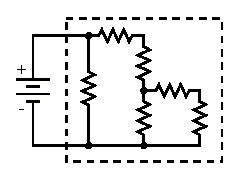
\includegraphics{rnetwork.eps}
    \caption{A resistor network powered by a voltage source.}
    \label{fig:rnetwork}
  \end{center}
\end{figure}

A \textbf{resistor network} is a collection of resistors connected
together as illustrated in Figure~\ref{fig:rnetwork}. Many resistor
networks can be reduced to a single resistance between two points using
Equations~\ref{eq:Rseries} and \ref{eq:Rparallel}. If a network can
be simplified in this way, the currents flowing through all of the
resistors in the network can be calculated by working backward through
the equivalent resistance calculation and applying the current
division expression of Equation~\ref{eq:Idiv} at each step.

If a network includes one or more $\Delta$ configurations --- three
resistors connected by junctions --- it cannot be simplified
via series and parallel pairs. A \textbf{junction} is a point in a
circuit where three or more wires meet. Junctions are marked with
$\bullet$ symbols in the schematics in these notes. However, any
$\Delta$ configuration in a network can be replaced with an equivalent
$Y$-shaped configuration via a $\Delta-Y$ transformation. This is easy
to look up. We won't concern ourselves with this situation.

%\vspace{12 pt}
%\noindent
%\fbox{\parbox{\linewidth-5\fboxsep}{
\begin{latexonly}
  \noindent
  \hrulefill
\end{latexonly}
\htmlrule
%\textbf{Resistor Network Analysis Summary}
\subsubsection*{Resistor Network Analysis Summary}
\begin{enumerate}
\item Use the equivalent resistance expressions
  (Equations~\ref{eq:Rseries} and \ref{eq:Rparallel}) to find the
  equivalent resistance of the entire network.

\item Use Ohm's law to calculate the current flowing through the
  voltage source.

\item Use the current division expressions
  (Equations~\ref{eq:Idiv}) at each node to determine the currents
  in the network.

\item Use Ohm's law to determine the voltage drops across the
  resistors and from these, the voltages of all of the nodes.
\end{enumerate}
\begin{latexonly}
  \noindent
  \hrulefill
\end{latexonly}
\htmlrule
%}}
  
\subsection{Kirchhoff's Rules}
\label{sec:kirchhoff}

Kirchhoff's Rules are used in the analysis of DC circuits and AC
circuits in the low-frequency limit --- in which magnetic induction
does not induce currents in the wires connecting elements in the
circuit.

The first rule, the \textbf{loop rule}, states that the total change
in electric potential around a closed loop must be zero. This means
that the sum of the potential differences across all of the devices in
a closed loop must be zero,
\begin{equation}
  \sum_\mathrm{loop} V_i = 0
  \label{eq:Loop}
\end{equation}
Signs are assigned to the $V_i$ according to the conventions
illustrated in Figure~\ref{fig:kirchhoffsigns}.

\begin{figure}[ht]
  \begin{center}
    \htmlimage{align='center'}{}
    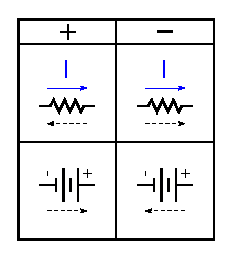
\includegraphics{kirchhoffsigns.eps}
    \caption{Sign conventions for the potential differences in
      Kirchhoff's loop rule equations. The blue arrows represent the
      direction of current flow. The black dashed arrows represent
      the direction the device is traversed in the process of
      generating the equation and therefore does not represent a
      physical quantity.}
    \label{fig:kirchhoffsigns}
  \end{center}
\end{figure}

The second rule, known as the \textbf{junction rule}, applies to
currents. This rule states that no net current enters or leaves a
junction,
\begin{equation}
  \sum_\mathrm{junction} I_i = 0
  \label{eq:junction}
\end{equation}
In the usual sign convention, currents flowing into a junction are
positive, and currents flowing out of a junction are negative. 

%\vspace{12 pt}
%\noindent
%\fbox{\parbox{\linewidth-5\fboxsep}{
\begin{latexonly}
  \noindent
  \hrulefill
\end{latexonly}
\htmlrule
%\textbf{Circuit Analysis using Kirchhoff's Rules}
\subsubsection*{Circuit Analysis using Kirchhoff's Rules}
\begin{enumerate}
\item Draw the circuit with arrows and labels representing all of
  the unique currents.
 
\item Construct a set of loop-rule equations including every
  device in the circuit at least once.

\item Construct a set junction-rule equations including every
  current in the circuit at least once.

\item Given enough known quantities (usually the properties of the
  devices in the circuit --- resistances, capacitances, source
  voltages, e.g.), these equations can be combined algebraically
  to determine the unknown quantities (usually currents and
  potential differences in the circuit).
\end{enumerate}
\begin{latexonly}
  \noindent
  \hrulefill
\end{latexonly}
\htmlrule
%  } }


\subsection{Th\'{e}venin's Theorem}
\label{sec:thevenin}
           
\begin{figure}[ht]
  \begin{center}
    \htmlimage{align='center'}{}
    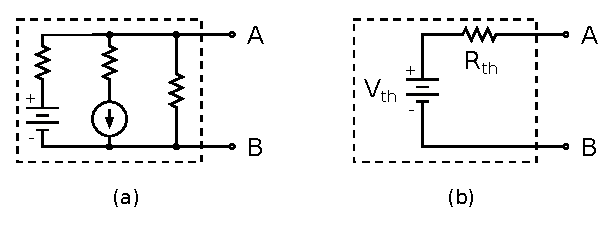
\includegraphics{thevenin.eps}
    \caption{Illustration of the Th\'{e}venin equivalent circuit (b) for a
      circuit (a) designed to drive a load connected across terminals A
      and B.}
    \label{fig:thevenin}
  \end{center}
\end{figure}

Any DC circuit consisting solely of resistors and voltage and current
sources can be replaced by a \textbf{Th\'{e}venin equivalent circuit}
consisting of a single DC voltage source in series with a resistor as
illustrated in Figure~\ref{fig:thevenin}. The theorem also applies to
the frequency response of AC circuits containing linear, passive
devices --- resistors, inductors, and capacitors.

%\vspace{12 pt}
%\noindent
%\fbox{\parbox{\linewidth-5\fboxsep}{
\begin{latexonly}
  \noindent
  \hrulefill
\end{latexonly}
\htmlrule
%\textbf{Finding the Th\'{e}venin Equivalent of a Circuit}
\subsubsection*{Finding the Th\'{e}venin Equivalent of a Circuit}
\begin{enumerate}
\item The Th\'{e}venin equivalent voltage $V_{th}$ is the voltage
  across the output terminals $A$ and $B$ of the circuit with no
  load attached.

\item The Th\'{e}venin equivalent resistance $R_{th}$ is the
  resistance of the circuit measured between the output terminals $A$
  and $B$, with all voltage and current sources replaced with
  their internal resistances. \textit{Ideal voltage sources have
    zero resistance, and ideal current sources have infinite
    resistance.}
\end{enumerate}
\begin{latexonly}
  \noindent
  \hrulefill
\end{latexonly}
\htmlrule
%} }

\newpage

\section{AC Circuits}
\label{sec:AC}

Alternating current (AC) circuits involve potential differences and
currents which vary periodically --- often sinusoidally --- with time.
The time-dependent response of an AC circuit to a sinusoidal driving
signal consists of a transient component that dies off due to
resistive losses, and a sinusoidal steady-state component. We will
focus on the steady-state behavior of the AC circuits we consider.

\subsection{Resistance, Reactance, and Impedance: the Complex Number 
  Representation}

When driven by a sinusoidal signal, the resulting currents through and
potential differences across capacitors, inductors, and resistors are
all sinusoidal as well, but with different, \textit{constant}, phase
relationships to each other.

%\vspace{12 pt}
%\noindent
%\fbox{\parbox{\linewidth-5\fboxsep}{
\begin{latexonly}
  \noindent
  \hrulefill
\end{latexonly}

\htmlrule
\noindent
\textbf{CIVIL}
\begin{quote}
The mnemonic CIVIL can be used to
remember that the voltage across a capacitor lags $\pi/2$ (half a
period of oscillation) behind the current (C\underline{IV}), and the
voltage across an inductor leads the current by $\pi/2$
(\underline{VI}L). The voltage across a resistor is always in phase
with the current.
\end{quote}
\htmlrule

\begin{latexonly}
  \noindent
  \hrulefill
\end{latexonly}
% }}
%\vspace{12 pt}

Ohm's law (Equation~\ref{eq:Ohm}) gives the full relationship between
current and voltage for a resistor. Capacitors and inductors are also
linear devices, but they impede the flow of current in the circuit
by temporarily storing energy in magnetic and electric fields instead
of by dissipating energy. We refer to these non-dissipative devices as
reactive devices, and we define quantities analogous to resistance
and which play the same role as resistance in a generalized version of
Ohm's law. The \textbf{inductive reactance} is given by
\begin{equation}
  X_L = j \omega L
  \label{eq:xl}
\end{equation}
where, $\omega = 2 \pi f$ is the driving frequency, and $L$ is the
inductance. In an electronics context,  $j$ is typically used to
represent $\sqrt{-1}$ instead of $i$ to avoid confusion with
current. The \textbf{capacitive reactance} 
\begin{equation}
  X_C = -\frac{j}{\omega C}
  \label{eq:xc}
\end{equation}
where $C$ is the capacitance. The factors of $j$ account for the
relative phases of the voltages and currents. Here, we are taking
advantage of the fact that the phase relationships between the
positive and negative imaginary axes and the real axis of the complex
plane map onto those between signals in inductors, capacitors, and
resistors, respectively.

Any network of linear devices ---  inductors, resistors, and
capacitors --- present a \emph{complex} \textbf{impedance} $Z$ to the
flow of current. The total impedance can be found by combining the
\emph{real} resistances and \emph{imaginary} reactances in the circuit
in the same way that we determined equivalent resistance in
Section~\ref{sec:serpar}. The inductive and capacitive reactances and
hence the total impedance $Z$ are frequency-dependent. In the
low-frequency limit, capacitors dominate the impedance, while in the
high-frequency limit, inductors dominate.

\subsection{Phasor Analysis}

We use complex numbers to represent impedance $Z$ and complex
functions to represent voltage and current as a bookkeeping
tool that simplifies the mathematics involved in circuit
analysis. The real-valued observable voltage and current are obtained
by  taking the real part of the complex voltage and current functions.
\begin{eqnarray}
  v(t) &=& Re(V \, e^{\,j\omega t + \phi_v}) = V \cos(\omega t + \phi_v)\\
  \nonumber
  i(t) &=& Re(I \, e^{\,j\omega t + \phi_i}) = I \cos(\omega t + \phi_i)
\end{eqnarray}
In many cases, we are only interested in the amplitudes $V$ and
$I$. In cases in which we do care about the phase, we typically
consider either $\phi_i$ or $\phi_v$ to be zero and keep track of the
relative phase.

The fact that complex voltage and current functions share an identical
time-dependent factor $e^{j \omega t}$, which cancels out of
equations that relate them, it is convenient to analyze AC circuits
using \textbf{phasors},
\begin{eqnarray}
  \mathbf{V} &=& V \, e^{\,j \phi_v}\\
  \nonumber
  \mathbf{I} &=& I \, e^{\,j \phi_i}
\end{eqnarray}
We can express the real voltage and current functions in terms of
phasors as
\begin{eqnarray}
  v(t) &=& Re(\mathbf{V} \, e^{\,j\omega t})\\
  \nonumber
  i(t) &=& Re(\mathbf{I} \, e^{\,j\omega t})
\end{eqnarray}
and the generalized version of Ohm's law becomes
\begin{equation}
  \mathbf{I} = \frac{\mathbf{V}}{Z}
  \label{eq:genohmphasor}
\end{equation}

The power in a component or network of components is given by
\begin{equation}
  \mathbf{P} = \mathbf{I^*V} = IV \, e^{\,j(\phi_v - \phi_i)}
  \label{eq:complexpower}
\end{equation}
The real part of the power is the power dissipated in resistors. The
imaginary part is the \textbf{reactive power} stored in capacitors and
inductors. Typically, we are interested in the average power
dissipated
\begin{equation}
  \left< P \right> = \frac{IV}{2} \cos(\phi_v - \phi_i)
                   = \frac{V^2}{2Z} \cos(\phi_v - \phi_i)
  \label{eq:rpower}
\end{equation}
The factor of 1/2 is the average value of $\cos^2(\omega t)$ ---
Equation~\ref{eq:rpower} gives the root mean square power.

Notice that if the relative phase $\phi_v - \phi_i$ is either $\pi/2$
or $-\pi/2$, no power is dissipated. These relative phases are only
possible if the impedance has no real part meaning there is no
resistance present.


%\vspace{12 pt}
%\noindent
%\fbox{\parbox{\linewidth-5\fboxsep}{
\begin{latexonly}
  \noindent
  \hrulefill
\end{latexonly}
\htmlrule
% \textbf{Phasor Analysis}
\subsubsection*{Phasor Analysis}
\begin{itemize}
\item Equivalent impedance calculations work the same way as
  equivalent resistance calculations (Equations~\ref{eq:Rseries}
  and \ref{eq:Rparallel}).

\item Kirchhoff's rules work for phasors $\mathbf{V}$ and
  $\mathbf{I}$.

\item Th\'{e}venin's theorem applies to AC circuits containing
  only linear components. The Th\'{e}venin voltage and impedance
  are found via the process outlined in Section~\ref{sec:thevenin}
  with impedance in place of resistance.
\end{itemize}
\begin{latexonly}
  \noindent
  \hrulefill
\end{latexonly}
\htmlrule
%  } }
%\vspace{12 pt}

\subsection{AC Voltage Dividers}
\label{sec:acvdiv}

\begin{figure}[ht]
  \begin{center}
    \htmlimage{align='center'}{}
    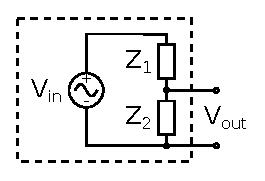
\includegraphics{acvdivider.eps}
    \caption{AC voltage divider between two linear devices, or networks of
      linear devices, with complex impedances $Z_1$ and $Z_2$.}
    \label{fig:acvdivider}
  \end{center}
\end{figure}

The AC voltage divider circuit shown in Figure~\ref{fig:acvdivider}
consists of two linear devices, which can be networks of linear
devices, with complex impedances $Z_1$ and $Z_2$. This is a series
circuit, so the current $\mathbf{I}$ flowing through all three
components is the same.

The loop rule equation
\begin{equation}
  \mathbf{V_{in}} - \mathbf{I} Z_1 - \mathbf{I} Z_2 = 0
\end{equation}
and the generalized Ohm's law for $Z_2$
\begin{equation}
  \mathbf{V_{out}} = \mathbf{I} Z_2
\end{equation}
combine to give
\begin{equation}
  \mathbf{V_{out}} = \frac{Z_2}{Z_1 + Z_2} \mathbf{V_{in}}
  \label{eq:vdivout}
\end{equation}

The real-valued amplitude of the output signal is the
magnitude of the phasor $\mathbf{V_{out}}$,
\begin{equation}
  V_{out} = \sqrt{\mathbf{V_{out}^* V_{out}}}
  \label{eq:vdivamp}
\end{equation}

\subsubsection*{Phase Angle}

The phase difference $\phi$ between $\mathbf{V_{out}}$ and
$\mathbf{V_{in}}$ is the \textbf{phase angle} between these complex
numbers in the complex plane. Since we are only looking for the 
\emph{difference}, we are free to set the complex phase of $\mathbf{V_{in}}$
to zero. This makes it easier to see that the only contribution to the
complex phase in Equation~\ref{eq:vdivout} comes from the impedances,
and that the phase angle of $\mathbf{V_{out}}$ relative to
$\mathbf{V_{in}}$ is determined by the real and imaginary parts of the
impedance ratio,
\begin{equation}
  \tan \phi = \frac{ Im \left( \frac{Z_2}{Z_1 + Z_2} \right) }
                   { Re \left( \frac{Z_2}{Z_1 + Z_2} \right) }
  \label{eq:vdivphase}
\end{equation}

\begin{quote}
  \textit{Note: The phase angle of an AC circuit is sometimes defined
    as the phase difference between $\mathbf{V_{in}}$ and
    $\mathbf{I}$, but we will Eq.~\ref{eq:vdivphase}, and these
    definitions are not in general equivalent.}
\end{quote}

\subsubsection*{Voltage Gain}

The \textbf{voltage gain} $A_V$ of the circuit is the ratio
$V_{out}/V_{in}$. It follows from Equation~\ref{eq:vdivout}
\begin{equation}
  A_V = \frac{V_{out}}{V_{in}} = \frac{|\mathbf{V_{out}}|}{|\mathbf{V_{in}}|}
                             = \left| \frac{Z_2}{Z_1 + Z_2} \right|
                             = \sqrt{ \left( \frac{Z_2}{Z_1 + Z_2} \right)^*
                                      \left( \frac{Z_2}{Z_1 + Z_2} \right) }
  \label{eq:gain}
\end{equation}
We sometimes refer to the ``3~dB point(s)'' of a circuit. These are
driving frequencies at which the \textit{power} gain is $\frac{1}{2}$,
which corresponds to voltage gain $A_v = \frac{1}{\sqrt{2}}$ (see
Appendix~\ref{sec:dB}).

\subsubsection*{Example: Series RLC Circuit}

\begin{figure}[ht]
  \begin{center}
    \htmlimage{align='center'}{}
    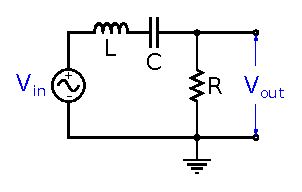
\includegraphics{rlccircuit.eps}
    \caption{A series RLC circuit as an AC voltage divider.}
    \label{fig:rlccircuit}
  \end{center}
\end{figure}

A series RLC circuit is shown in Figure~\ref{fig:rlccircuit}. We will
treat this as a voltage divider between the series inductor-capacitor
pair and the resistor. The resistor is by itself in the lower part of
the divider, so $Z_2 = R$. The inductor and capacitor are connected in
series, so we combine their reactances as we would series resistances
(Equation~\ref{eq:Rseries})
\begin{equation}
  Z_1 = j \left( \omega L - \frac{1}{\omega C} \right)
\end{equation}

Equation~\ref{eq:gain} becomes
\begin{equation}
  \frac{V_{out}}{V_{in}} = \sqrt{\frac{R^2}{R^2 + (\omega L - 1/\omega C)^2}}
\end{equation}
To evaluate the phase angle, it is helpful to put the
impedance ratio in Equation~\ref{eq:vdivamp} in $a + jb$ form by
multiplying the numerator and denominator by the complex conjugate of
the denominator
\begin{equation}
  \frac{Z_2}{Z_1 + Z_2}
  = \frac{R}{R + j \left( \omega L - \frac{1}{\omega C} \right)}
  = \frac{R^2 - j R \left( \omega L - \frac{1}{\omega C} \right)}
         {R^2 + \left( \omega L - \frac{1}{\omega C} \right)^2}
\end{equation}
which, with Equation~\ref{eq:vdivphase}, gives
\begin{equation}
  \tan \phi = \frac{\frac{1}{\omega C} - \omega L}{R}
\end{equation}

Figure~\ref{fig:rlcscope} illustrates the
potential differences across the resistor $v_{out}(t)$ and the AC
voltage source $v_{in}(t)$ as they would appear on an oscilloscope. 
The phase angle $\phi$ is proportional to the time difference $\Delta t =
t_{V_{out}} - t_{V_{in}}$ between the two signals, illustrated in
panel (a) of the figure, as 
\begin{equation}
  \Delta t = \frac{\phi}{\omega} = \frac{\phi}{2 \pi f} = \frac{\phi}{2 \pi} T
  \label{eq:deltatphi}
\end{equation}
where $T$ is the period of oscillation of the input signal.

\begin{figure}[ht]
  \htmlimage{align='center'}{}
  \begin{center}
    \scalebox{0.45}{
      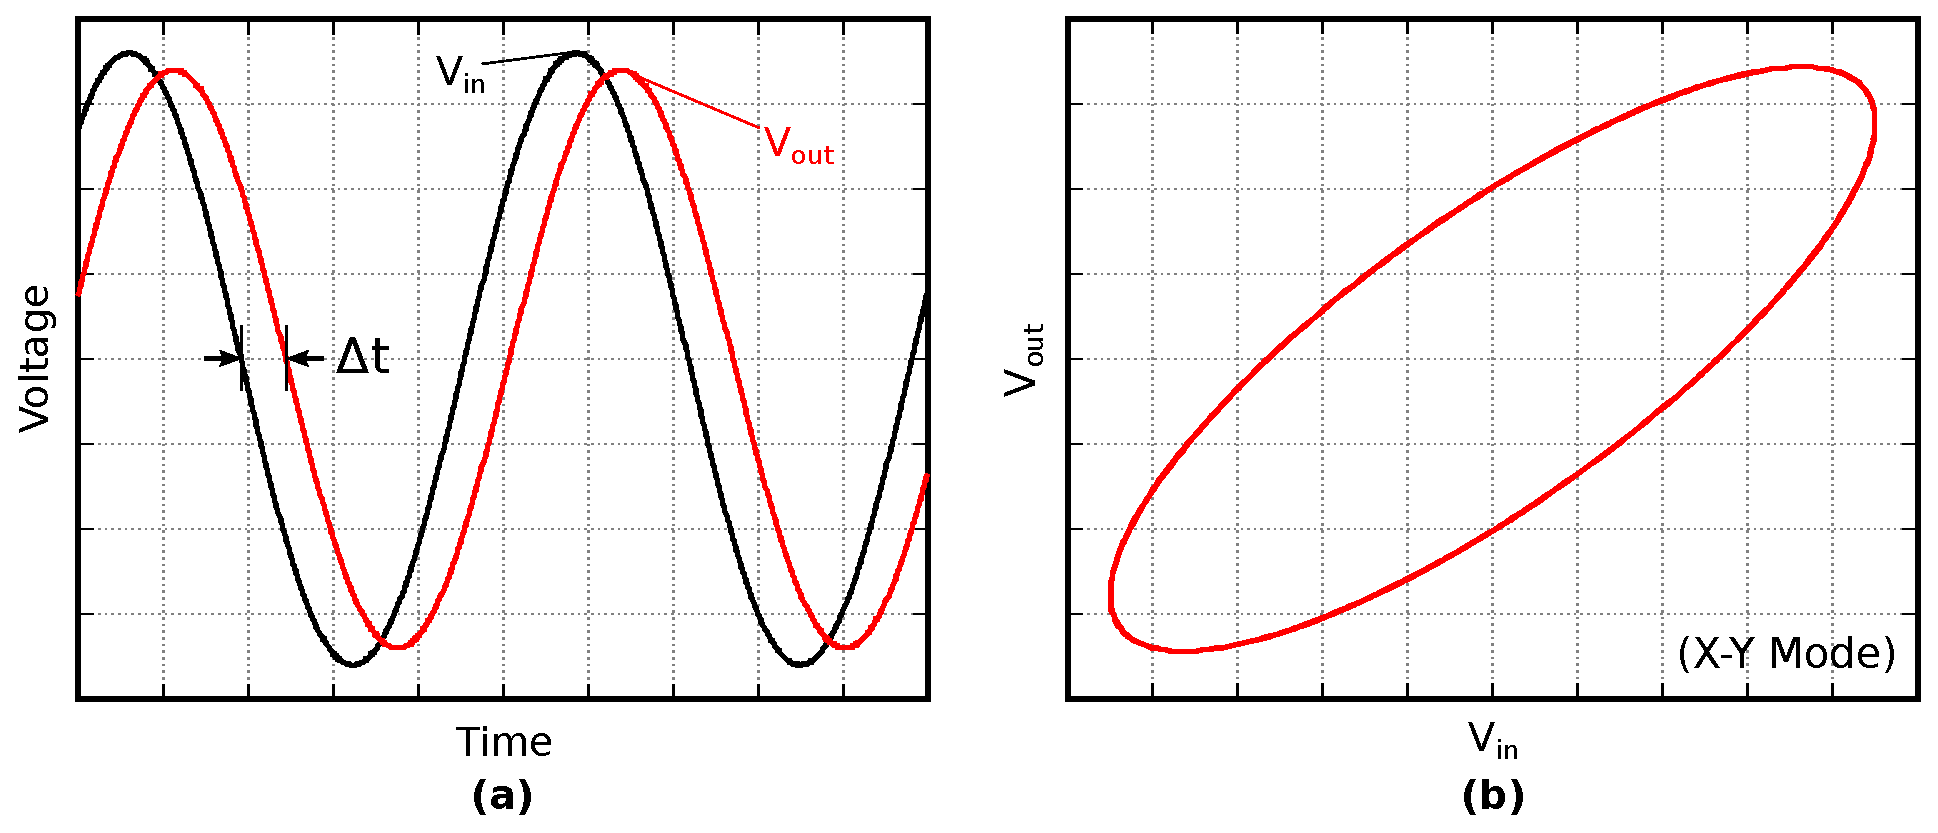
\includegraphics{rlcnr.eps}
    }
    \vspace{12 pt}
    \scalebox{0.45}{
      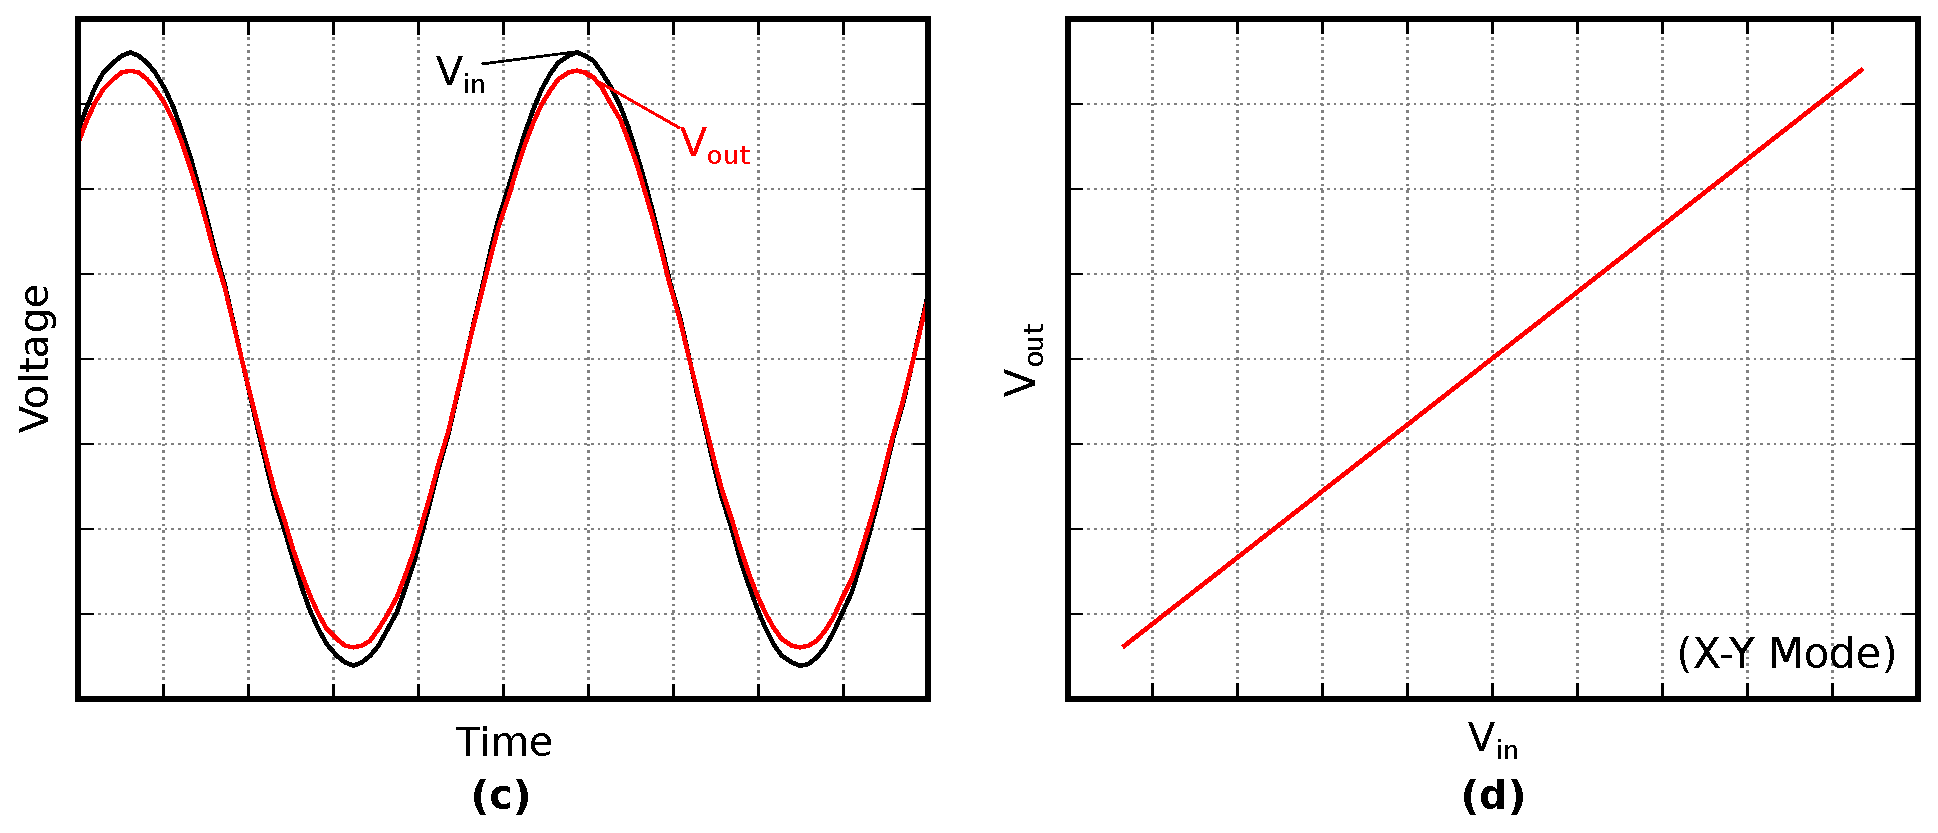
\includegraphics{rlcres.eps}
    }
    \caption{Oscilloscope displays of the potential differences across the
      resistor and AC power source in the series RLC voltage divider shown in 
      Figure~\ref{fig:rlccircuit}. Panels (a) and (b) show the potential
      vs. time and X-Y mode displays for the circuit at a non-resonant
      driving frequency. Panels (c) and (d) show the same displays at the
      resonant frequency $\omega_o$ of the circuit.}
    \label{fig:rlcscope}
  \end{center}
\end{figure}

\begin{figure}[ht]
  \htmlimage{align='center'}{}
  \begin{center}
    \scalebox{0.45}{
      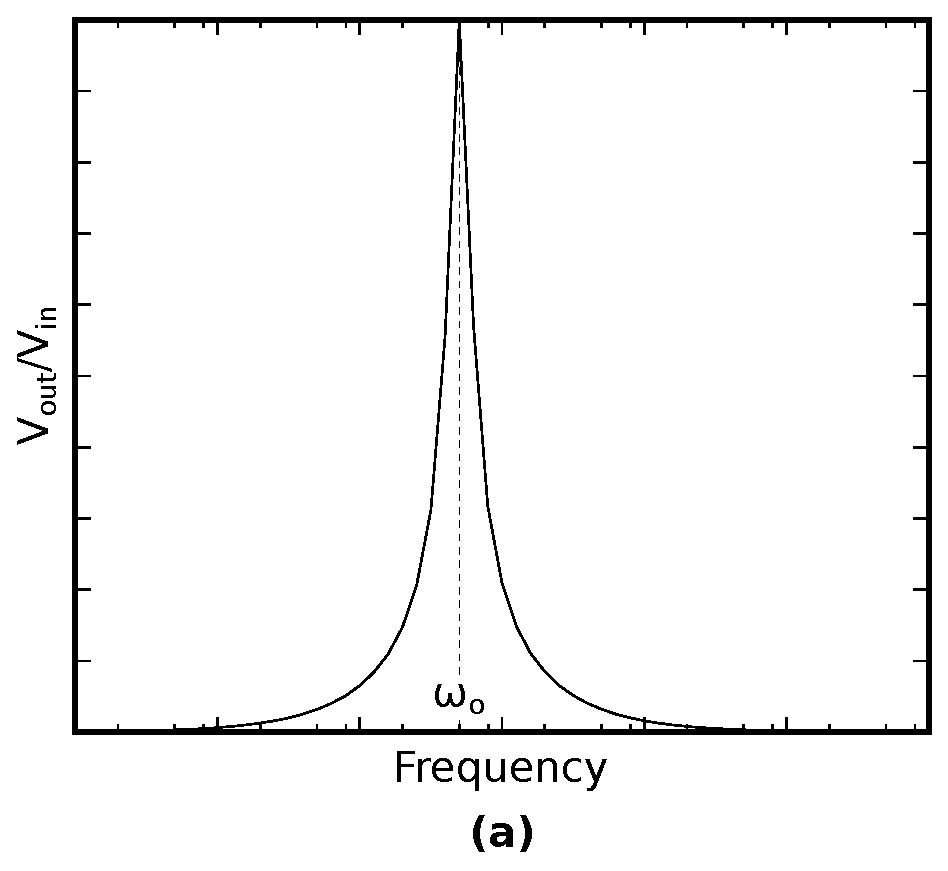
\includegraphics{rlc_vout.eps}
    }
    \hspace{12 pt}
    \scalebox{0.45}{
      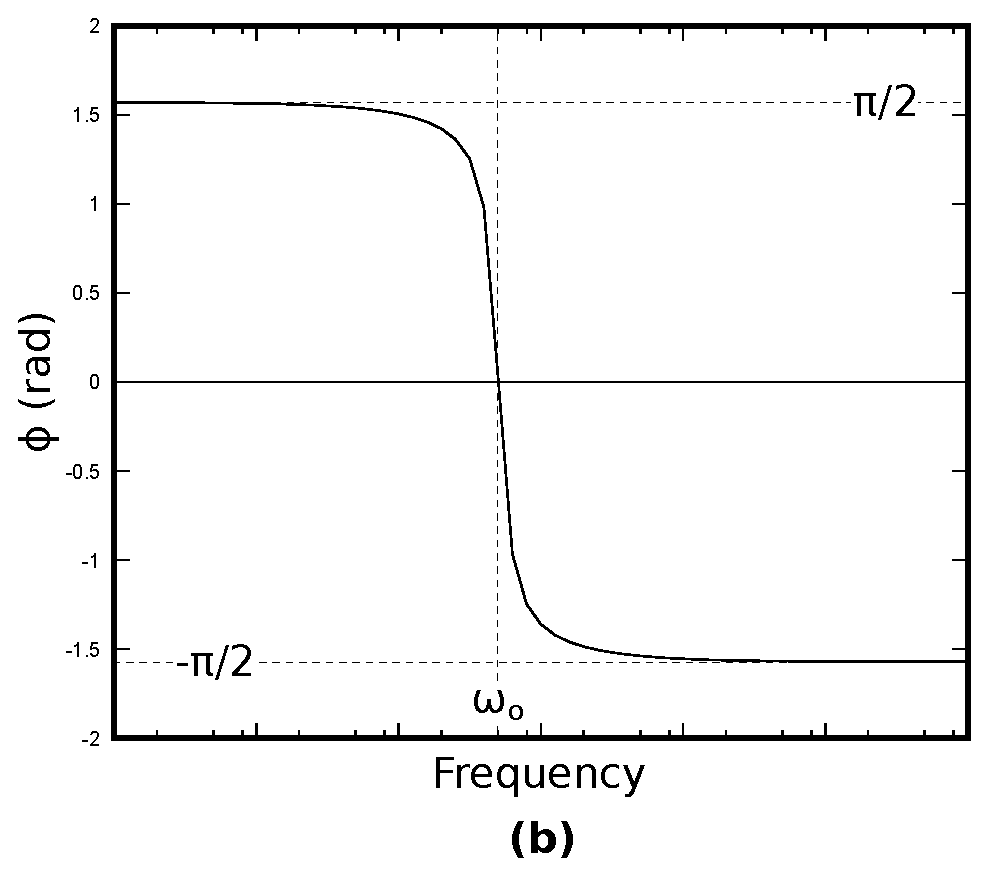
\includegraphics{rlc_phi.eps}
    }
    \caption{Frequency response --- (a) gain $V_{out}/V_{in}$ and (b)
      phase angle $\phi$ --- of the series RLC voltage divider shown in 
      Figure~\ref{fig:rlccircuit}. Note that frequency is on a log scale 
      in both plots.}
    \label{fig:rlcvphi}
  \end{center}
\end{figure}

There is a special frequency, called the \textbf{resonant frequency}
$\omega_o$ of the circuit, at which 
the impedance $Z_1$ of the inductor-capacitor pair goes to zero, the
current $I$ is maximal, $V_{out} = V_{in}$ and the phase angle
$\phi$ is zero. Combining Equations~\ref{eq:xl} and \ref{eq:xc} to
find the the frequency at which the capacitive and inductive
reactances $X_L$ and $X_C$ have equal magnitudes and cancel out,
yields  
\begin{equation}
  \omega_o = \frac{1}{\sqrt{LC}}
  \label{eq:rlcomega}
\end{equation}
Panels (c) and (d) of Figure~\ref{fig:rlcscope} illustrate the
potential differences across the resistor $v_{out}(t)$ and the AC
source $v_{in}(t)$ at resonance. The plots show $V_{out}$ slightly
less than $V_{in}$ at resonance due to the internal resistance of a
non-ideal inductor.

Figure~\ref{fig:rlcvphi} illustrates the frequency response of the
circuit. The \textbf{voltage gain} $A_V = V_{out}/V_{in}$ is plotted
in panel (a) and the phase angle $\phi$ is plotted in panel (b). This
circuit acts as a \textbf{band pass filter}. It transmits the input
signal in a range of frequencies. The phase angle plot shows that the
impedance is dominated by the capacitor at low frequencies and by the
inductor at high frequencies as we would expect based on the frequency
dependence of the respective reactances (Equations~\ref{eq:xl} and 
\ref{eq:xc}).

We can also make sense of the qualitative behavior of the phase angle
using the CIVIL mnemonic. At low frequencies, where the capacitor
dominates, we expect the current to lead the voltage across the
capacitor (C\underline{IV}). In this circuit, $v_{out}$ is the voltage
across the resistor, which is in phase with the current, so we expect
a positive phase angle at low frequencies. At high frequencies, the
inductor dominates, and the current lags behind the voltage across the
inductor (\underline{VI}L). This gives a negative phase
angle. \emph{Which of these situations is illustrated in panel (a) of
  Figure~\ref{fig:rlcscope}?}

\newpage

\section{Diodes}
\label{sec:diodes}

\begin{figure}[ht]
  \htmlimage{align='center'}{}
  \begin{center}
    \scalebox{0.5}{
      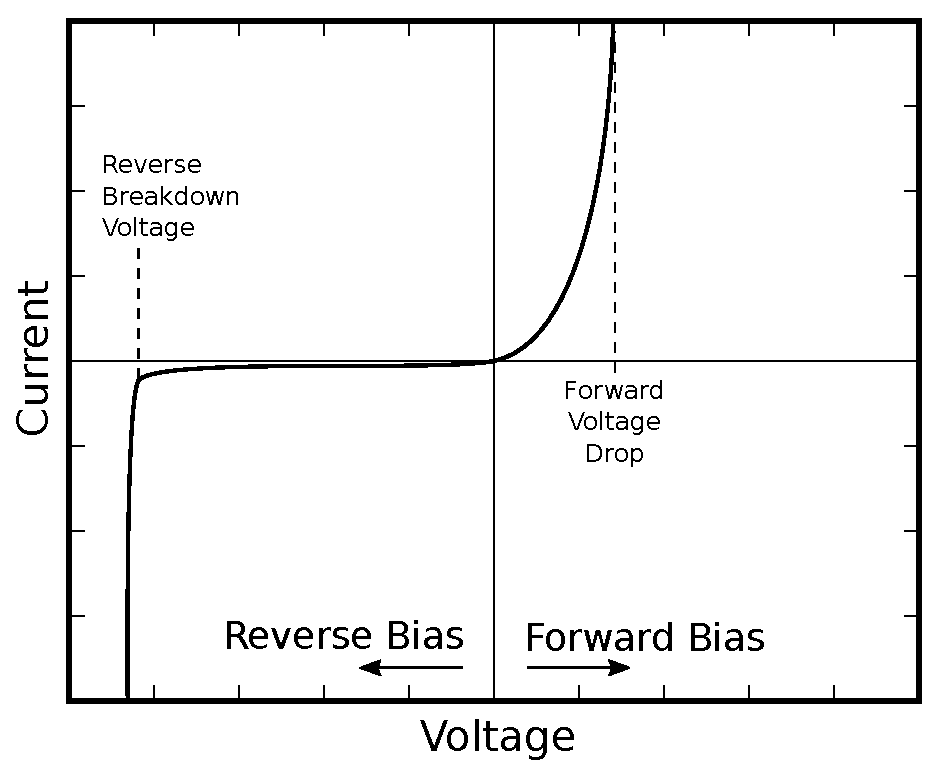
\includegraphics{diodevi.eps}
    }
    \caption{\emph{Qualitative} V-I curve for a standard diode. \emph{The
        scale on the reverse-bias side of the graph is roughly two orders
        of magnitude larger than the forward-bias side.}}
    \label{fig:diodevi}
  \end{center}
\end{figure}

Diodes are non-Ohmic, passive devices containing a junction between
p-type and n-type semiconductor. The n-type (negative) region contains
extra electrons and the p-type (positive) region contains extra
electron vacancies. Electrons diffuse from the n-type region into the
p-type region, and electron-vacancies in the p-type region diffuse
into the n-type region, creating an electric field pointing toward the
p-type region. The region of field is called the \textbf{depletion
  region}. The electric field in the depletion region acts as a
``hill'' in the potential-energy landscape. When a potential
difference is applied to the device oriented to create an electric
field in the ``uphill'' direction, toward the n-type region, the hill
is reduced in height, and if the applied potential difference is
larger than the height of the hill, called the \textbf{forward 
  voltage drop}, current flows through the junction.  If
a potential difference is applied creating an electric field in the
``downhill'' direction, the height of the hill is increased, and the
flow of current is blocked. There is a maximum ``downhill'' potential 
difference called the \textbf{reverse breakdown voltage} beyond which
current flows backward across the junction. This damages standard diodes.
The $V$ vs. $I$ curve of a standard diode is sketched qualitatively in
Figure~\ref{fig:diodevi}. The forward voltage drop and reverse
breakdown voltage are labeled in the figure. The arrow in the
schematic symbol for a diode (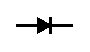
\includegraphics{diode.eps}) points in
the ``forward'' direction. 

Standard diodes are designed to operate between the reverse breakdown
voltage and the forward bias voltage. At the forward bias voltage,
also called the \textbf{diode drop}, a diode behaves essentially like
a wire with a built-in voltage drop. If a bias voltage below the diode
drop (and above the reverse breakdown voltage) is applied, an ideal diode
behaves essentially like an open switch or an infinite
resistance. However, in a real diode, a tiny \textbf{leakage current}
flows, as indicated by the shallow slope of the $V-I$ curve above
breakdown in the reverse-bias region of
Figure~\ref{fig:diodevi}. The standard silicon diodes you will encounter
in lab have forward voltage drops of about 0.7~V, reverse
breakdown voltages of 100-1000 V, and leakage currents on the order of
$10^{-8}$~A.

\newpage

\section{Transistors}
\label{sec:transistors}

\begin{figure}[ht]
  \htmlimage{align='center'}{}
  \begin{center}
    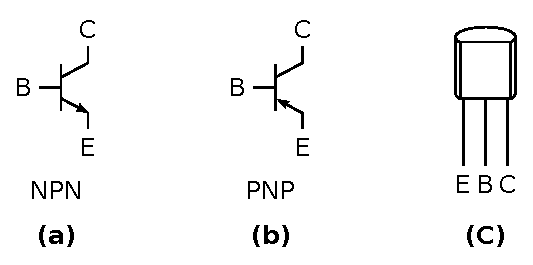
\includegraphics{transistors.eps}
    \caption{Schematic symbols for (a) NPN and (b) PNP bipolar junction
      transistors with labels on the collector (C), base (B), and
      emitter (E). (c) The plastic TO-92 transistor package we will use
      in lab with pins labeled.}
    \label{fig:transistors}
  \end{center}
\end{figure}

A \textbf{transistor} is an \textbf{active device}, meaning that it
enables the control of a current by an input signal. There are several
different types of transistors, each suited to different
applications. Here, we will focus on
\textbf{bipolar junction transistors} (BJTs).
Transistors have three terminals called the \textbf{emitter}, the
\textbf{collector}, and the \textbf{base}. A BJT consists of two
p-type -- n-type junctions, like those in a diode. In an NPN
transistor, the base is p-type semiconductor, and the emitter and
collector are n-type. In a PNP transistor, the polarities are
reversed. 

Schematic symbols for BJTs and an illustration of the ordering of the
pins on the transistors we will use in lab are shown in
Figure~\ref{fig:transistors}. The arrows on the schematic symbols
indicate the direction of the collector current $I_C$.

\subsection{Transistor Behavior}

Transistors operate in one of three states, which we will refer to
here as ``off'', ``on'' (also ``saturation''), and the ``active
region.'' In amplifiers, transistors operate in the active region. In
digital and switching applications, transistors rapidly transition
between ``off'' and ``on'' states. Transistors in voltage regulators
stay in the the ``on'' state.

\subsubsection*{Active Region}

The \textbf{Ebers-Moll equation} describes the relationship between
the collector current $I_C$ and the voltage drop from base to emitter
$V_{BE}$ by 
\begin{equation}
  I_C = I_o \left( e^{\frac{V_{BE}}{kT/e}} - 1 \right)
  \label{eq:ebersmoll}
\end{equation}
where $I_o$ is the reverse leakage current from the emitter to the
base, $e = 1.6 \times 10^{-19}$~C is the elementary unit of charge,
$k = 1.38 \times 10^{-23}$~J/K is the Boltzmann constant, and $T$ is the
absolute temperature (in Kelvin). With typical doping levels, the
leakage current arising from the ``intrinsic'' behavior of the pure
semiconductor is very small, and the second term (-$I_o$) is
negligible, giving a simple exponential dependence of $I_C$ on
$V_{BE}$.

\begin{figure}[ht]
  \htmlimage{align='center'}{}
  \begin{center}
    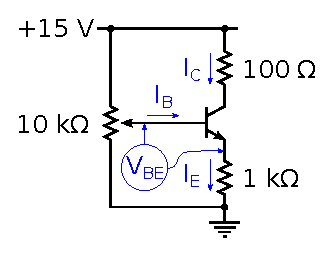
\includegraphics{ebersmollcircuit.eps}
    \caption{Schematic of the circuit you will use in lab to
      test the Ebers-Moll equation in the active region of an NPN
      BJT.}
    \label{fig:ebersmollcircuit}
  \end{center}
\end{figure}

This current-voltage relationship is the same as for the diode,
plotted qualitatively in Figure~\ref{fig:diodevi}. We usually operate
diodes in \textbf{saturation}, at the forward voltage drop ($\approx
0.7$~V for silicon pn junctions). In some applications, like the
transistor switch described in Section~\ref{sec:transistorswitch}, we
operate transistors in the same way. Below saturation in the
\textbf{active region}, we need the Ebers-Moll equation to model
transistor behavior. The schematic of the circuit you will use in lab
to investigate the Ebers-Moll equation is shown in
Figure~\ref{fig:ebersmollcircuit}. The variable resistor enables you
to adjust $V_{BE}$ from 0~V to saturation. The 100~$\Omega$ resistor
gives you a way to determine the collector current $I_C$ from a
voltage measurement, and the 1~k$\Omega$ resistor keeps the collector
and emitter currents under control to protect the transistor.

In the active region, the $V_{BE}$ vs. $I_C$ curve has a small,
nonzero slope, which manifests itself as a small emitter resistance,
\begin{equation}
  r_e = \frac{d V_{BE}}{d I_C} = \frac{kT/e}{I_C}
\label{eq:emitterresistance}
\end{equation}
which at room temperature is $(25~\Omega)/I_C[\mathrm{mA}]$.

\subsubsection*{Transistor On (Saturation)}

In a bipolar junction transistor, the diode drop across the
collector-base junction is smaller than that of the base-emitter
junction.  This means that when a transistor is operating in
\textbf{saturation}, the voltage drop from collector to emitter
$V_{CE}$ is smaller than $V_{BE}$.  For a standard silicon transistor
in saturation, $V_{CE} \approx 0.25$~V.

In saturation, the collector current $I_C$ is greater than the current
flowing from the base to the collector $I_B$ by a factor $h_{FE}$,
which is on the order of 100 and depends on temperature,
\begin{equation}
  I_C = h_{FE} I_B
  \label{eq:hfe}
\end{equation}

\subsubsection*{Transistor Off}

When $V_{BE}$ is significantly below 0.7~V, the exponential in
Equation~\ref{eq:ebersmoll} is orders of magnitude smaller than its
saturation value, and the collector and emitter currents $I_C$ and
$I_E$ are effectively turned off. 

For a given transistor, there are maximum rated values of $I_C$,
$I_B$, and $V_{CE}$. If these values are exceeded, the transistor will
fail. You might wonder, given the exponential relationship between
$V_{BE}$ and the collector current $I_C$ of
Equation~\ref{eq:ebersmoll}, what keeps the current from growing
beyond a safe level and destroying the transistor. When we operate a
transistor in saturation, where the exponential really takes off,
other devices in the circuit must limit the current, and we don't need
to think about where we are on the exponential curve. The same is true
for diodes.

%\vspace{12 pt}
%\noindent
%\fbox{\parbox{\linewidth-5\fboxsep}{
\htmlrule
\begin{latexonly}
  \noindent
  \hrulefill
\end{latexonly}
%\textbf{Basic Transistor Behavior}
\subsubsection*{Basic Transistor Behavior}
\begin{itemize}
\item In order for a transistor to function, make $V_C > V_E$, and
  keep $I_B$, $I_C$, and $V_{CE}$ below the rated maximum
  values of the transistor.

\item \textbf{On:} In saturation, $V_{BE} \approx 0.7$~V,
  $V_{CE} \approx 0.25$~V, and $I_C = h_{FE} I_B$, where
  $h_{FE} \approx 100$. 

\item \textbf{Off:} If $V_{BE} < 0.7$~V (significantly),
  $I_C \approx 0$.

\item \textbf{Active Region:} $V_{BE}$ is between ``off'' and
  saturation. The collector current is governed by the Ebers-Moll
  equation (Equation~\ref{eq:ebersmoll}). The emitter resistance
  at room temperature is $r_e = (25~\Omega)/I_C[\mathrm{mA}]$.
\end{itemize}
\begin{latexonly}
  \noindent
  \hrulefill
\end{latexonly}
\htmlrule
%}}

\subsection{Application: Transistor Switch}
\label{sec:transistorswitch}

\begin{figure}[ht]
  \htmlimage{align='center'}{}
  \begin{center}
    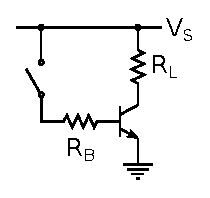
\includegraphics{transistorswitch.eps}
    \caption{Schematic of a transistor switch circuit in which a small
      base current is used to deliver a larger current to a load.}
    \label{fig:transistorswitch}
  \end{center}
\end{figure}

The circuit shown in Figure~\ref{fig:transistorswitch} implements a
transistor as a switch controlling power delivered to the load
resistance $R_L$.  Closing the mechanical switch drives a current from
the base to the emitter.  With a proper choice of $R_B$, the base
current is large enough to saturate the transistor, bringing the base
voltage to $\approx0.7$~V.  The collector current produces a voltage
drop across $R_L$ of $\approx V_S$. The collector voltage is very close to
the emitter ($\approx 0.25$~V), and the right branch of the circuit
behaves as if the collector is grounded. Opening the switch
brings $V_{BE}$ significantly below 0.7~V, and the transistor shuts
off power to the load.

What the point of this? Why not dispense with the transistor, and put
the switch in series with the load, as is the case with household
wiring? In applications in which the control switch is far away from a
load that draws a large current, it is safer to run small 
control currents over long distances and keep the large currents close
to the load.

\subsubsection*{Design}

\begin{enumerate}
\item Set the supply voltage $V_S$ to provide the current required by
  the load. The transistor will operate in saturation, so the
  collector-emitter voltage drop will be only $\approx 0.25$~V, and
  the remainder of $V_S$ will drive the load.

\item Choose a transistor rated to handle the required base current
  and power drawn by the load.
  
\item Set the value of $R_B$ to keep the transistor in saturation
  while delivering the maximum desired current under all
  circumstances. Given possible variations in $R_L$ and the range
  of $h_{FE}$ among the make/model of transistor used (see the data
  sheet from the manufacturer), it is generally good to use a generous
  base current ($\approx 10~I_C/h_{fe}$).

  \emph{As long as the supply voltage $V_S$ is appropriate to the
    load, the load resistance will limit the current, so it does no
    harm to deliver a larger base current than is absolutely required,
    as long as it does not exceed the rated maximum base current.}
\end{enumerate}

\subsection{Application: Emitter Follower}
\label{sec:emitterfollower}

\begin{figure}[ht]
  \htmlimage{align='center'}{}
  \begin{center}
    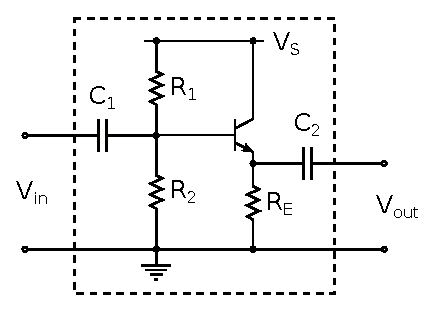
\includegraphics{emitterfollower.eps}
    \caption{Schematic of an AC coupled emitter follower.}
    \label{fig:emitterfollower}
  \end{center}
\end{figure}

An \textbf{emitter follower} is a power amplifier. It has a
voltage gain of $A_v \approx 1$ and a large current gain. It is useful
in applications in which a load that draws high power is driven by a
small signal --- audio amplifiers, for example.
The schematic of an AC coupled emitter follower is shown in
Figure~\ref{fig:emitterfollower}. 

\subsubsection*{Design}

\begin{enumerate}
\item The emitter voltage $V_E$ is limited between ground and the
  source voltage $V_S$. Choose an emitter resistance $R_E$ to center
  the quiescent\footnote{The term \textbf{quiescent} refers to the
    state of the circuit when the input signal is not varying.}
  emitter voltage in this range, at the average current
  drawn by the load. Centering $V_E$ allows the output signal vary in
  a symmetrical range.

\item Once $V_E$ is established, set the values of the input bias
  resistors $R_1$ and $R_2$.
  \begin{enumerate}
  \item Their ratio $R_1/R_2$ must place $V_{BE}$ in the active region
    of the transistor ($V_B \approx V_E + 0.6~\mathrm{V}$).

  \item Their parallel resistance must be small compared with that
    presented by the base-emitter junction so that they do not drag 
    down the quiescent current $R_1 || R_2 \approx h_{FE} R_E/ 10$. 
  \end{enumerate}

\item The capacitors $C_1$ and $C_2$ are coupling capacitors that
  remove DC components from the input and output signals. They, along
  with the resistors in the input and output stages, act as high-pass 
  filters. Their values are chosen such that they do not filter out
  frequencies of interest.
\end{enumerate}

\subsection{Application: Common Emitter Amplifier}
\label{sec:commonemitter}

\begin{figure}[ht]
  \htmlimage{align='center'}{}
  \begin{center}
    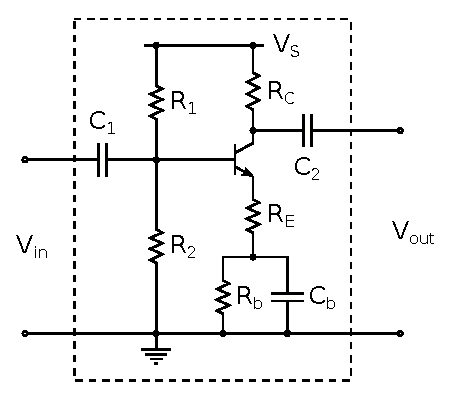
\includegraphics{commonemitter.eps}
    \caption{Schematic of an AC coupled common emitter amplifier.}
    \label{fig:commonemitter}
  \end{center}
\end{figure}

A \textbf{common emitter amplifier} is an inverting voltage
amplifier. The schematic of an AC coupled common emitter amplifier is
shown in Figure~\ref{fig:commonemitter}.
It has a voltage gain given by
\begin{equation}
  A_v = -\frac{R_C}{R_E}
  \label{eq:commonemittergain}
\end{equation}

\subsubsection*{Design}

\begin{enumerate}
\item The collector resistor $R_C$ is chosen to center the collector
  voltage between ground and $V_S$ at the desired quiescent current.

\item The emitter resistor $R_E$ is chosen to give the desired voltage
  gain (Equation~\ref{eq:commonemittergain}).

  \emph{Keep in mind that the emitter resistance $r_e$ in series with
    $R_E$ acts to reduce the measured voltage gain relative to the
    prediction of Equation~\ref{eq:commonemittergain}. The emitter
    resistance can be estimated using
    Equation~\ref{eq:emitterresistance} with the quiescent collector
    current.}

\item The bias resistor $R_b$ is set to place the quiescent emitter
  voltage at about 1~V.

  \emph{This greatly reduces the influence of the
    temperature-dependent (and very small) emitter resistance $r_e$ on
    the stability of the quiescent base-emitter voltage $V_{BE}$,
    which must be kept in the active region of the transistor.}

\item The bypass capacitor $C_b$ is chosen to give very small
  capacitive reactance ($\approx \frac{R_b}{10}$ at the lowest signal 
  frequency, thus shorting out the bias resistor so that only $R_E +
  r_e$ remain, yielding the desired voltage gain.

\item Once the emitter voltage $V_E$ is established, set the values of
  the input bias resistors $R_1$ and $R_2$.
  \begin{enumerate}
  \item Their ratio $R_1/R_2$ must place $V_{BE}$ in the active region
    of the transistor ($V_B \approx V_E + 0.6~\mathrm{V}$).

  \item Their parallel resistance must be small compared with that
    presented by the base-emitter junction so that they do not drag 
    down the quiescent current
    $R_1 || R_2 \approx h_{FE} (R_E + R_b)/10$.
  \end{enumerate}

\item The values of the coupling capacitors $C_1$ and $C_2$ are chosen
  so that they allow frequencies of interest to pass through. The
  input coupling capacitor $C_1$ and $R_1||R_2$ act as a
  high-pass filter on the input. Similarly, $C_2$ and $R_C||(R_E +
  R_b)$ act as a high-pass filter on the output. 
\end{enumerate}

\newpage

\section{Operational Amplifiers (Op Amps)}
\label{sec:opamps}

\begin{figure}[ht]
  \htmlimage{align='center'}{}
  \begin{center}
    \scalebox{0.7}{
      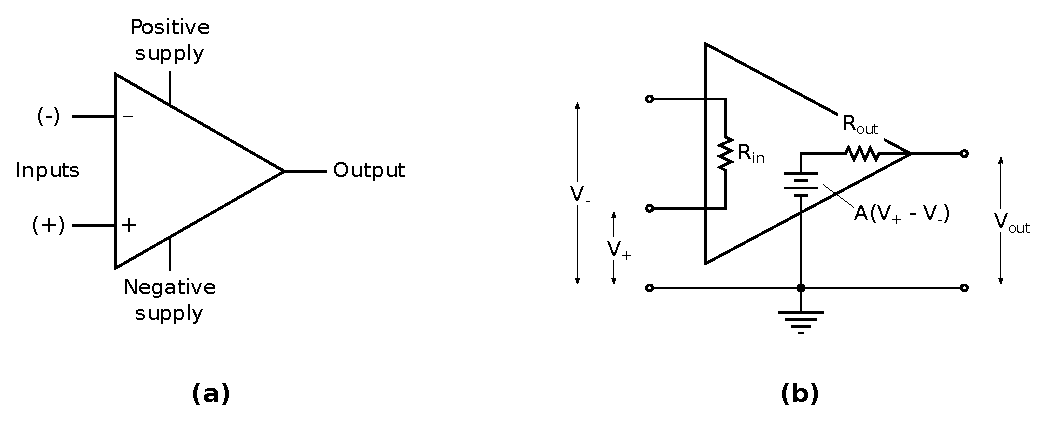
\includegraphics{opamp_model.eps}
    }
    \caption{(a) Schematic symbol of an operational amplifier, and
      (b) a circuit model of an op amp.}
    \label{fig:opampmodel}
  \end{center}
\end{figure}

We considered simple transistor amplifiers in
Sections~\ref{sec:emitterfollower} and \ref{sec:commonemitter}.
Amplifier circuits with nice properties --- high gain and 
high input impedance, for example --- packaged as integrated circuits
(ICs), are called \textbf{operational amplifiers} or op amps. They are
called ``operational'' amplifiers, because they can be used to perform
arithmetic operations like addition, subtraction, and multiplication
with signals. In fact, op amps can also be used to integrate and
differentiate signals.

The schematic symbol for an op amp is shown in panel (a)
of Figure~\ref{fig:opampmodel}. A circuit model of an op amp is shown
in panel (b) of Figure~\ref{fig:opampmodel}. The output voltage of the
op amp is linearly proportional to the voltage difference between the
inverting and non-inverting input terminals $V_+ - V_-$ by a factor of
the gain $A$. However, the output voltage is limited to the range
$-V_S \leq V_{out} \leq V_S$, where $V_S$ is the supply voltage. The
range $-V_S < V_{out} < V_S$ is often called the \textbf{linear region}
of the amplifier, and when the output swings to $V_S$ or $-V_S$, the
op amp is said to be \textbf{saturated}. The output voltages of the
transistor amplifiers described in Sections~\ref{sec:emitterfollower} and
\ref{sec:commonemitter} are similarly limited by the supply voltage.

An ideal op amp has infinite gain ($A = \infty$), infinite input
resistance ( $R_{in} = \infty$), and zero output resistance
($R_{out} = 0$). You should use these assumptions to analyze op amp
circuits. A consequence of the assumption of infinite gain is that, if
the output voltage is within the finite linear region, we must have
$V_+ = V_-$. A real op amp has a gain in the range $10^3$-$10^5$,
depending on the type, and hence actually maintains a very small
difference in input terminal voltages when operating in its linear
region. For most applications, we can get away with assuming
$V_+ \approx V_-$. If the positive or negative input of an op amp is
connected directly to ground, the other input will be held very close
to ground and can be considered grounded in circuit analysis. This is
referred to as a \textbf{virtual ground}.

%\vspace{12 pt}
%\noindent
%\fbox{\parbox{\linewidth-5\fboxsep}{
\htmlrule
\begin{latexonly}
  \noindent
  \hrulefill
\end{latexonly}
%\textbf{Basic Op Amp Behavior}
\subsubsection*{Basic Op Amp Behavior}
\begin{itemize}
\item $R_{in} = \infty,~A = \infty,~R_{out} = 0$
\item \textbf{Linear region:} $V_+ = V_-,~-V_S < V_{out} < V_S$
\item \textbf{Saturation:} $V_+ > V_-~~\Longrightarrow~~V_{out} = V_S$
  ~~~or~~~ $V_+ < V_-~~\Longrightarrow~~V_{out} = -V_S$
\end{itemize}
\htmlrule
\begin{latexonly}
  \noindent
  \hrulefill
\end{latexonly}
%}}
%\vspace{12 pt}

We stock two operational amplifiers in the lab, the \texttt{LM741}, a
general purpose bipolar junction transistor (BJT) based amplifier with
a typical input resistance of 2 M$\Omega $, and the \texttt{LF411},
with field effect transistors (FETs) at the inputs giving a much
larger input resistance ($10^{12}~\Omega$). Data sheets for these
devices are available on the Texas Instruments web site
(\url{www.ti.com}). Of the two, the \texttt{LF411} comes closest to
satisfying the assumptions associated with ideal op amp behavior. It
costs more than the \texttt{LM741} (\$1.84 vs. \$0.94 as of fall
2021).

\subsection{Application: Inverting Amplifier}
\label{sec:invertingamp}

\begin{figure}[ht]
  \htmlimage{align='center'}{}
  \begin{center}
    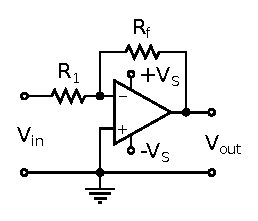
\includegraphics{invertingamp.eps}
    \caption{Schematic of an op amp based inverting amplifier.}
    \label{fig:invertingamp}
  \end{center}
\end{figure}

In op amp based inverting amplifier is shown in
Figure~\ref{fig:invertingamp}. The analysis of the behavior of the
circuit is based on two very good approximations.
\begin{enumerate}
\item There is a virtual ground at the inputs of the op-amp.
  
\item The very large input impedance of the op amp means that it
  draws negligible current. Therefore, the current $I$ flowing through
  the input resistor $R_1$ is the same as that flowing through the
  feedback resistor $R_f$.
\end{enumerate}
It follows that
\begin{equation}
  I = \frac{V_{in}}{R_1} = \frac{-V_{out}}{R_f}
\end{equation}
which gives a voltage gain of
\begin{equation}
  A_v = -\frac{R_f}{R_1}
  \label{eq:invampgain}
\end{equation}

The input resistor $R_1$ is connected directly to the virtual ground,
so the input resistance of the circuit is $R_1$. The output resistance
is $R_{oa}||R_f$, where $R_{oa}$ is the very small output resistance
of the op amp.

\emph{The inverting amplifier has the advantage of low noise due to
  the lower input impedance, relative to a non-inverting amplifier. It
  also has a relatively fast \textbf{slew rate}, the maximum rate of
  change of the signal.}

\subsubsection*{Design}
\begin{enumerate}
\item The value of $R_1$ is chosen to give the desired input
  impedance.

\item The ratio $R_f/R_1$ is fixed by the desired voltage gain
  (Equation~\ref{eq:invampgain}).
\end{enumerate}

\subsection{Application: Non-inverting Amplifier}
\label{sec:noninvertingamp}

\begin{figure}[ht]
  \htmlimage{align='center'}{}
  \begin{center}
    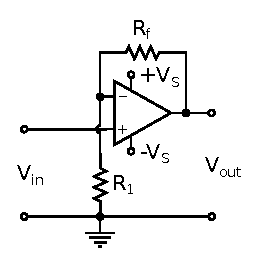
\includegraphics{noninvertingamp.eps}
    \caption{Schematic of an op amp based non-inverting amplifier.}
    \label{fig:noninvertingamp}
  \end{center}
\end{figure}

An op amp based non-inverting amplifier is shown in
Figure~\ref{fig:noninvertingamp}.

The feedback loop of this amplifier is delivered by a voltage divider
in which $V_{out}$ is split by resistors $R_f$ and $R_1$ and delivered
to the negative input of the op amp, so that $V_{in}$ and $V_{out}$
are related by the voltage division expression
\begin{equation}
  V_{in} = \frac{R_1}{R_1 + R_f} V_{out}
\end{equation}
which gives a voltage gain of
\begin{equation}
  A_v = 1 + \frac{R_f}{R_1}
  \label{eq:noninvampgain}
\end{equation}

The input is connected directly to the positive input of the op amp,
so the input resistance of the circuit is that of the op amp. The
output resistance is $R_{oa}||(R_1 + R_f)$, where $R_{oa}$ is the very
small output resistance of the op amp.

\emph{The non-inverting amplifier has the advantages of the op amp
  itself, large input impedance and small output impedance. It has the
  disadvantage that it is susceptible to positive feedback to the
  non-inverting input from via $R_f$ which can lead to saturation.}

\subsubsection*{Design}
\begin{enumerate}
\item The ratio $R_f/R_1$ is fixed by the desired voltage gain
  (Equation~\ref{eq:noninvampgain}).

\item The absolute values of $R_f$ and $R_1$ are chosen to be large enough
  that the amplifier does not draw too much power and low enough that
  noise is not a problem. (The 10~k$\Omega$ - 500~k$\Omega$ range is
  reasonable.)
\end{enumerate}

\subsection{Application: Voltage Follower/Buffer}
\label{sec:vfollower}

\begin{figure}[h!]
  \htmlimage{align='center'}{}
  \begin{center}
    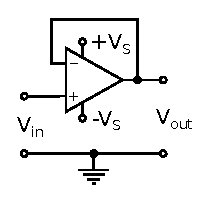
\includegraphics{vfollower.eps}
    \caption{Schematic of an op amp based voltage follower/buffer.}
    \label{fig:vfollower}
  \end{center}
\end{figure}

The voltage follower or buffer, shown in Figure~\ref{fig:vfollower},
is a special case of the non-inverting amplifier of
Section~\ref{sec:noninvertingamp} with $R_1 = \infty$ and $R_f = 0$, 
giving a voltage gain of $A_v = 1$.
This is useful for mirroring signals from low-power sources at the
output of the op amp, which has very small output impedance and can
deliver higher power.

\subsection{Application: Summing Amplifier}
\label{sec:summingamp}

\begin{figure}[h!]
  \htmlimage{align='center'}{}
  \begin{center}
    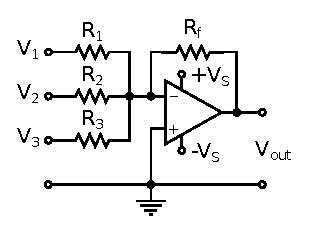
\includegraphics{summingamp.eps}
    \caption{Schematic of an op amp based summing amplifier.}
    \label{fig:summingamp}
  \end{center}
\end{figure}

An op amp based summing amplifier is shown in
Figure~\ref{fig:summingamp}. The analysis of the circuit is very
similar to that of the inverting amplifier in
Section~\ref{sec:invertingamp}, with the additional complexity of
multiple inputs. The virtual ground at the op-amp inputs gives simple
expressions for the currents,
\begin{eqnarray}
  \label{eq:sumampI1}
  I_1 &=& \frac{V_1}{R_1}\\
  I_2 &=& \frac{V_2}{R_2}\\
  I_3 &=& \frac{V_3}{R_3}\\
  I_f &=& \frac{V_{out}}{R_f}
\end{eqnarray}
which combine according to the junction rule at the inputs of
the op amp
\begin{equation}
  \label{eq:sumampjunction}
  I_1 + I_2 + I_3 = I_f
\end{equation}
Combining Eqs.~\ref{eq:sumampI1} - \ref{eq:sumampjunction} yields the
output voltage 
\begin{equation}
  \label{eq:summingampvout}
  V_{out} = -\left( \frac{R_1}{R_f} V_1 + \frac{R_2}{R_f} V_2
                 + \frac{R_3}{R_f} V_3 \right)  
\end{equation}

As we would expect based on the analysis of the inverting amplifier in
Section~\ref{sec:invertingamp}, the input resistance ``seen'' by each
input signal is that of the corresponding input resistor.  The output
resistance is $R_{oa}||R_f$, where $R_{oa}$ is the very small output
resistance of the op amp.

\subsubsection*{Design}
\begin{itemize}
\item The ratios $R_1/R_f$, $R_1/R_f$, and $R_1/R_f$ are determined by
  the desired coefficients of the output sum
  (Eq.~\ref{eq:summingampvout}).

\item The absolute values of the resistors are chosen to give 
  acceptable input resistances.

\end{itemize}

\subsection{Application: Differential Amplifier}
\label{sec:differentialamp}

\begin{figure}[h!]
  \htmlimage{align='center'}{}
  \begin{center}
    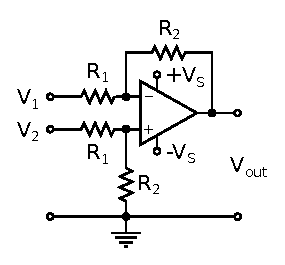
\includegraphics{differenceamp.eps}
    \caption{Schematic of an op amp based differential amplifier.}
    \label{fig:differenceamp}
  \end{center}
\end{figure}

An op amp based differential amplifier is shown in
Figure~\ref{fig:differenceamp}. The analysis of the circuit can be
done using the junction rule for the virtual junction at the
op-amp inputs
\begin{equation}
  I_1 + I_2 = I_3 + I_4
\end{equation}
where the four unique currents carried by the resistors are
\begin{eqnarray}
  \label{eq:differentialI1}
  I_1 &=& \frac{V_1 - V_-}{R_1}\\
  I_2 &=& \frac{V_2 - V_+}{R_1}\\
  I_3 &=& \frac{V_- - V_{out}}{R_2}\\
  I_4 &=& \frac{V_+}{R_2}
\end{eqnarray}
combined with the voltage division expression for the positive input,
\begin{equation}
  \label{eq:differentialVplus}
  V_+ = \frac{R_2}{R_1 + R_2} V_2
\end{equation}
Combining Eqs.~\ref{eq:differentialI1} - \ref{eq:differentialVplus}
with the assumption the $V_- = V_+$ gives the output voltage 
\begin{equation}
  V_{out} = - \frac{R_2}{R_1} \left(V_1 - V_2\right)
\end{equation}

\subsubsection*{Design}
\begin{itemize}
\item The ratio $R_1/R_2$ is determined by the desired voltage gain.

\item Matching the values of the two $R_1$ resistors and the two $R_2$
  resistors is important to getting the gain right. Moreover, if $V_1$
  and $V_2$ have a common DC component, mismatched resistors will
  introduce a DC component to the output.

\end{itemize}

\subsection{Application: Differentiator}
\label{sec:differentiator}

\begin{figure}[h!]
  \htmlimage{align='center'}{}
  \begin{center}
    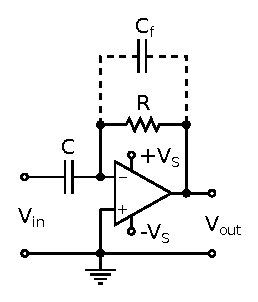
\includegraphics{differentiator.eps}
    \caption{Schematic of an op amp based differentiator.}
    \label{fig:differentiator}
  \end{center}
\end{figure}

An op amp based differentiator is shown in
Figure~\ref{fig:differentiator}. The optional feedback capacitor $C_f
< C$ is often needed to damp oscillations in the output. The following
analysis ignores $C_f$.

This circuit has a virtual ground at the op-amp inputs. It follows
that 
\begin{equation}
  \label{eq:differentiatorvout}
  V_{out} = - IR
\end{equation}
and also that the charge on the capacitor is related to the input
voltage by
\begin{equation}
  V_{in} = \frac{Q}{C}
\end{equation}
The current $I$ flowing through the resistor is to a good
approximation equal to that of the capacitor, which we can relate to
the charge on the capacitor via the definition of current
\begin{equation}
  \label{eq:differentiatorI}
  I \equiv \frac{dQ}{dt}
\end{equation}
Combining Eqs.~\ref{eq:differentiatorvout} - \ref{eq:differentiatorI}
yields 
\begin{equation}
  \label{eq:opampdiff}
  V_{out} = - RC \frac{d V_{in}}{dt}
\end{equation}

\subsubsection*{Design}
\begin{itemize}
\item The values of $R$ and $C$ are chosen to roughly match the
  desired time scale $RC$ of the differentiation. 

\item If high-frequency oscillation is observed in the output, the
  feedback capacitor is needed. Its value is set to damp the
  oscillation without also damping the desired output.
  
\end{itemize}

\subsection{Application: Integrator}
\label{sec:integrator}

\begin{figure}[h!]
  \htmlimage{align='center'}{}
  \begin{center}
    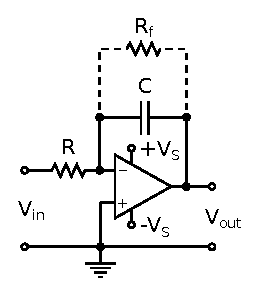
\includegraphics{integrator.eps}
    \caption{Schematic of an op amp based integrator.}
    \label{fig:integrator}
  \end{center}
\end{figure}

An op amp based integrator circuit is shown in
Figure~\ref{fig:integrator}. The optional feedback resistor $R_f$ is
needed to drain the feedback capacitor in order to prevent the
saturation of the op amp. The feedback resistor is ignored in the 
following analysis.

This circuit has a virtual ground at the op-amp inputs. It follows
that the current flowing through the input resistor is related to the
input voltage by
\begin{equation}
  \label{eq:integratorI}
  I = \frac{V_{in}}{R}
\end{equation}
and the charge on the capacitor is related to the output voltage by 
\begin{equation}
  \label{eq:integratorVout}
  V_{out} = -\frac{Q}{C}
\end{equation}
Using the definition of current ($I \equiv dQ/dt$),
Eq.~\ref{eq:integratorI} can be integrated to find the charge on the
capacitor.
\begin{equation}
  \label{eq:integratorQ}
  Q = \int dQ = \frac{1}{R} \int V_{in} \, dt
\end{equation}
Combining Eqs.~\ref{eq:integratorVout} and \ref{eq:integratorQ} yields 
\begin{equation}
  \label{eq:opampint}
  V_{out} = - \frac{1}{RC} \int V_{in} \, dt
\end{equation}

\subsubsection*{Design}
\begin{itemize}
\item The values of $R$ and $C$ are chosen to roughly match the
  desired time scale $RC$ of the integration. 

\item The value of the feedback resistor $R_f$ is chosen to discharge
  the feedback capacitor on an acceptable time scale without distorting
  the output of the integrator.
  
\end{itemize}

%% \subsection{Application: Schmitt Trigger}
%% \label{sec:schmitt}

%% \begin{figure}[h!]
%%   \begin{center}
%%     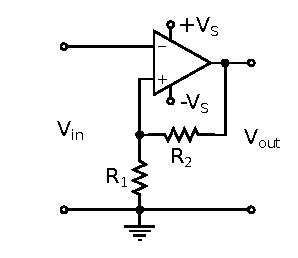
\includegraphics{schmitt.eps}
%%     \caption{Schematic of an op amp based inverting Schmitt trigger.} 
%%     \label{fig:schmitt}
%%   \end{center}
%% \end{figure}

%% A Schmitt trigger is a two-state system that
%% switches to an ``on'' value at its output when the input crosses a high
%% voltage threshold $V_+$ and switches to an ``off'' value when the
%% input crosses a low voltage threshold $V_-$. 

%% An op amp based inverting Schmitt trigger circuit is shown in
%% Figure~\ref{fig:schmitt}. The ``on'' and ``off'' values of the circuit
%% are close to $V_{on} = -V_S$ and $V_{off} = +V_S$, respectively. It is
%% an inverting Schmitt trigger, because its ``on'' value is negative and
%% its ``off'' value is positive.

%% The thresholds of the circuit are determined by the voltage division
%% of $V_{out}$ by resistors $R_1$ and $R_2$. When the trigger is
%% operating, it is in saturation either at $V_{out} = V_S$ or
%% $V_{out} = -V_S$. The voltage division expressions are therefore
%% \begin{equation}
%%   \label{eq:schmittVplus}
%%   V_+ = \frac{R_1}{R_1 + R_2} V_S
%% \end{equation}
%% and
%% \begin{equation}
%%   \label{eq:schmittVminus}
%%   V_- = - \frac{R_1}{R_1 + R_2} V_S
%% \end{equation}

%% \subsubsection*{Design}
%% \begin{itemize}
%% \item The relative values of $R_1$ and $R_2$ are chosen to give the
%%   desired thresholds (Eqs.~\ref and \ref).

%% \item The absolute values of $R_1$ and $R_2$ are chosen to avoid
%%   dragging down the load.
  
%% \end{itemize}

%===========================================================================

\clearpage
\appendix

\section{Reading Electronics Schematics}
\label{sec:schematics}

\subsubsection*{Schematic Symbols}

\begin{figure}[ht]
  \htmlimage{align='center'}{}
  \begin{center}
    \scalebox{0.8}{
      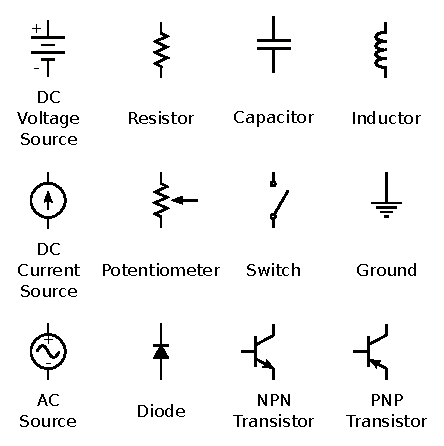
\includegraphics{schematic.eps}
    }
   \end{center}
  \caption{Schematic symbols.}
  \label{fig:schematics}
\end{figure}

The schematic symbols used in these notes are shown in
Figure~\ref{fig:schematics}. An adjustable component, like the
variable capacitor in a tuner circuit, is represented with the
standard symbol with an arrow through it: 
\begin{center}
  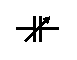
\includegraphics{var_capacitor.eps}
\end{center}

\subsubsection*{An Example}

\begin{figure}[ht]
  \htmlimage{align='center'}{}
  \begin{center}
    \scalebox{0.8}{
      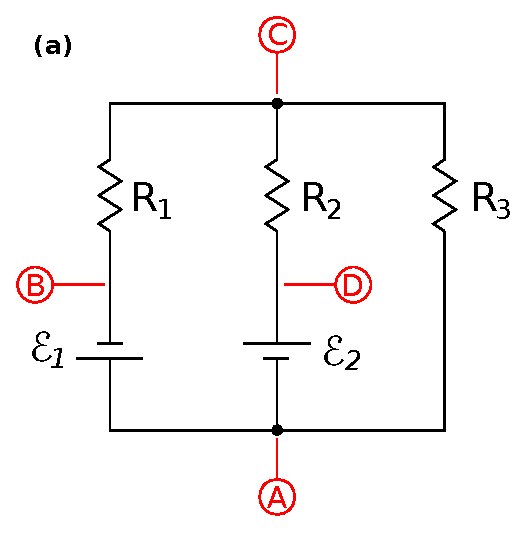
\includegraphics{schematic_example.eps}
    }\\
    \vspace{12 pt}
    \scalebox{0.8}{
      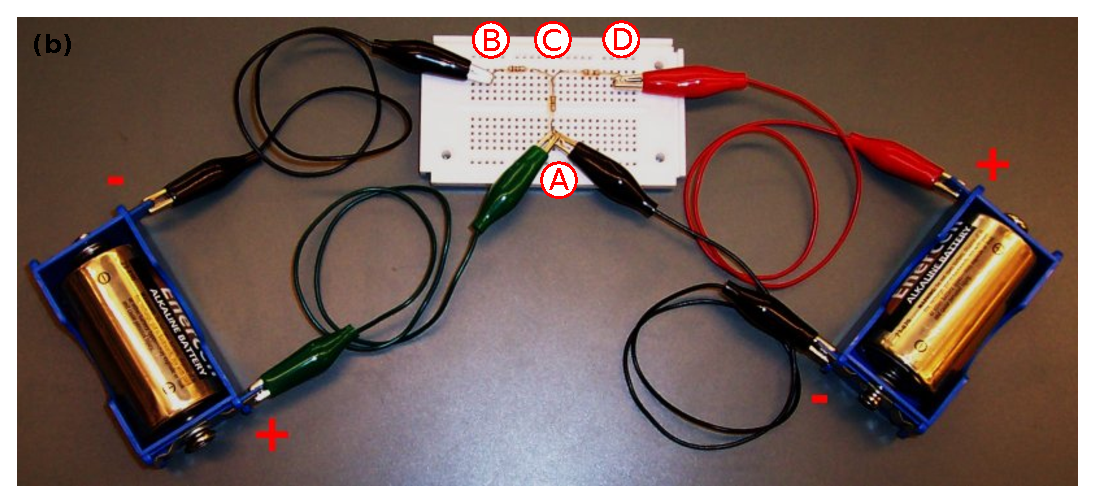
\includegraphics{schematic_example_image.eps}
    }
   \end{center}
  \caption{(a) Example of an electronics schematic. (b) One way 
    the circuit might really look.}
  \label{fig:schematic_example}
\end{figure}

An electronics diagram or \textbf{schematic} is designed to
communicate a specific way of connecting electronics components.
Lines between components represent wires. Schematics usually have a
rectangular layout, but this layout rarely represents how things are
oriented in reality. Nothing is drawn to scale. Wires can follow
curved three-dimensional paths. Components  can be oriented
differently than they appear. All that really matters is the way
components are wires are connected. For example, a circuit schematic is
shown in Figure~\ref{fig:schematic_example}(a), and one way a real
version of the circuit might look is shown in
Figure~\ref{fig:schematic_example}(b). 

\subsubsection*{Junctions and Branches}

It is useful to pay attention to points in a circuit where three or
more wires meet in a circuit. These are called
\textbf{junctions}. They are important in circuit  
analysis, because currents combine or divide at these points. They are
marked with $\bullet$ symbols in the schematics in these notes.
Junctions are connected by \textbf{branches}. A branch might
contain multiple wires and components, but in carries a single
current, because all of the components and wires in a branch are
connected in series. In single-loop circuits, there are no junctions
--- a single current flows through all components. There are two
junctions and three branches in the example circuit in
Figure~\ref{fig:schematic_example}. It follows from the latter that
there are three unique currents flowing in the circuit.

\section{The Breadboard}
\label{sec:breadboard}

\begin{figure}[ht]
  \htmlimage{align='center'}{}
  \begin{center}
    \scalebox{0.5}{
      \includegraphics{breadboard.eps}
    }
    \caption{Schematic of a breadboard with shaded rectangles showing
      conducting connections between the sockets.}
    \label{fig:breadboard}
  \end{center}
\end{figure}

A \textbf{breadboard} allows for easy, temporary assembly and
modification of a circuit by sliding components and wires into the
various sockets. The sockets are linked in an easily recognizable
pattern that allows for the components and wires to be connected in a
circuit. This pattern is indicated by the shaded rectangles in
Figure~\ref{fig:breadboard}.  The long distribution strips in the
figure are meant for conveniently distributing power to
components. These strips must be connected to power sources. They can
also be used to distribute a connection to a common ground.  The
terminal strips are connected in groups of five. They are not
connected across the channel. Integrated circuits (ICs) can be plugged
in across the channel so that each pin is connected to a single
terminal strip to allow for easy connections to other components.

\section{Resistor Color Codes}

\begin{figure}[ht]
  \htmlimage{align='center'}{}
  \begin{center}
    %% Latex2html doesn't recognize the colortabl package, so...
    %%\begin{tabular}{|r|c|c|c|c|c|c|c|c|c|c|c|}\hline
    %%\bf color      & \color{white}\cellcolor{Black}black & \color{white}\cellcolor{Brown}brown & \cellcolor{Red}red & \cellcolor{Orange}orange & \cellcolor{Yellow}yellow & \cellcolor{Green}green & \cellcolor{Blue}blue &
    %%\cellcolor{Purple}violet & \cellcolor{Gray}gray & white \\\hline
    %%\bf digit      & 0     & 1     & 2   & 3      & 4      & 5     & 6    &
    %%7      & 8    & 9     \\\hline
    %%\bf multiplier & 1     & 10    & 100 & 1k     & 10k    & 100k  & 1M   &
    %%10M    & 100M & 1000M \\\hline
    %%\end{tabular}
    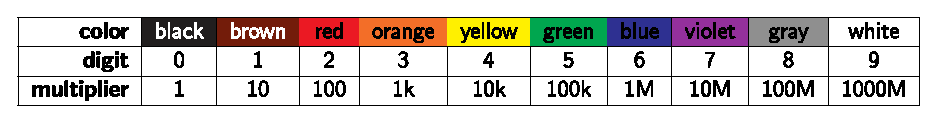
\includegraphics{resistor_color_codes.eps}
    \begin{eqnarray*}
      R = [\mathrm{band 1}][\mathrm{band 2}] 
      \times 10^{[\mathrm{band 3}]} & \pm & 5\%~(\mathrm{gold})\\ 
      & \pm & 10\%~(\mathrm{silver})\nonumber
    \end{eqnarray*}
    \caption{\label{fig:rcolorcodes} Guide to resistor color codes.}
  \end{center}
\end{figure}

Most resistors you will encounter are marked with a set of bands,
according to a standard color code, summarized in
Figure~\ref{fig:rcolorcodes}, which you can use to determine their
resistances. There are ten colors corresponding to numerical digits
0-9 (See the table below.), and gold and silver bands indicating 5\%
and 10\% accuracy in the coded resistance, respectively.  Starting at
the far end of the resistor from the gold/silver band, the first two
bands are the first two digits in the resistance.  The third band
gives the power of ten by which you multiply the first two digits to
obtain the resistance. For example, Blue Yellow Red Gold gives $R = 64
\times 10^{2}~\Omega = 64 \times 100~\Omega = 6400~\Omega$ with a
tolerance of 5\%, or $\pm 320~\Omega$.

\section{Digital Multimeter (DMM) Guide}
\label{sec:dmm}

\begin{figure}[ht]
  \htmlimage{align='center'}{}
  \begin{center}
    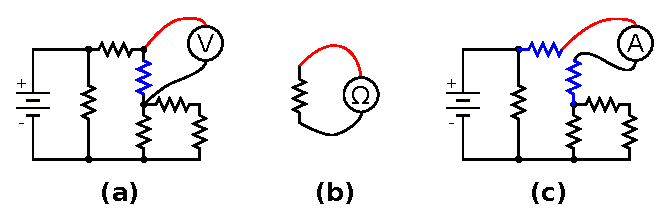
\includegraphics{dmm.eps}
    
    \caption{Schematics illustrating how a multimeter is connected to
      measure (a) the voltage drop across the resistor highlighted in
      blue, (b) the resistance of a resistor, and (c) the current
      flowing through the branch of the circuit highlighted in blue.}
    \label{fig:dmm}
  \end{center}
\end{figure}

\subsection{Measuring Potential Difference (Voltage Drop)}

\begin{itemize}
\item Plug the probes into the \texttt{COM} and \texttt{V\,$\Omega$}
  ports on the DMM.

\item Switch the DMM to one of the voltage scales.
  
\item Connect the DMM in parallel with the resistor as shown in panel
  (a) of Figure~\ref{fig:dmm}, and it will display the measured
  potential difference.

\item Find the voltage scale that gives you the most
  precise reading --- the one with the upper bound larger than, but
  closest to, the measured potential difference.
\end{itemize}

\subsection{Measuring Resistance}

\emph{The resistor must not be connected to a circuit while you are
  measuring its resistance.}

\begin{itemize}
\item Plug the probes into the \texttt{COM} and \texttt{V\,$\Omega$}
  ports on the DMM.

\item Switch the DMM to one of the resistance scales.
  
\item Connect the DMM leads to the leads of the resistor as illustrated in
  panel (b) of Figure~\ref{fig:dmm}, and it will display the measured
  resistance.

\item Find the resistance scale that gives you the most
  precise reading --- the one with the upper bound larger than, but
  closest to, the measured resistance.
\end{itemize}

\subsection{Measuring Current}

\emph{Never connect the DMM in parallel with anything while measuring
  current. In current-measuring mode, the resistance of the DMM is
  very small, and it acts as a wire. Connecting the DMM in parallel
  with a component will short it out, possibly drawing enough current
  to blow a fuse in the DMM.}

\begin{itemize}
\item Plug the probes into the \texttt{COM} and current ports of the
  DMM. There are two current ports (usually labeled \texttt{A} and
  \texttt{mA} with their maximum current ratings). Choose the one
  appropriate to the current you plan to measure. When in doubt, use
  the high current port, and switch to the more sensitive one if you
  determine that the current is low enough.

\item Switch the DMM to one of the current scales corresponding to the
  current port you are using.

\item Connect the DMM in series with the branch of the circuit through
  which you want to measure the current as illustrated in panel (c) of
  Figure~\ref{fig:dmm}.
  
\item Find the current scale that gives you the most precise reading
  --- the one with the upper bound larger than, but closest to, the
  measured current.
\end{itemize}

\section{Decibels}
\label{sec:dB}

It is convenient, when comparing two quantities, call them $Thing_1$ 
and $Thing_2$, that differ by several orders of magnitude, to use a
logarithmic scale for the comparison. One such approach is the
\textbf{decibel scale}.
\begin{equation}
  dB = 10 \log \left( \frac{\mathrm{Thing_2}}{\mathrm{Thing_1}} \right)
  \label{eq:db}
\end{equation}
For example, if $\mathrm{Thing_2}$ is $10^8$ times larger than
$\mathrm{Thing_1}$, we can say $\mathrm{Thing_2}$ is 80~dB above
$\mathrm{Thing_1}$. Where $\mathrm{Thing_2}$ is the intensity
of sound in an environment, and $\mathrm{Thing_1}$ is the threshold of
human hearing ($10^{-12}$~W/m$^2$), this is called the
\textbf{sound level}.

In the electronics context, we use decibels to compare signal
amplitude and power. Often, the \textbf{3~dB point} is used to characterize 
electronic filters. That is the frequency at which the power
transmitted by the filter is reduced by a factor 2 relative to the
incident power 
\[
10 \log \left( \frac{P_{out}}{P_{in}} \right)
= 10 \log \left( \frac{1}{2} \right) = 10 (-0.3010) = -3.01
\]
The power is proportional to the square of the voltage, so the 3~dB
point is the frequency (or frequencies) at which the voltage gain
$|V_{in}|/|V_{out}|$ is $1/\sqrt{2}$. 

%% \section{OrCAD Capture}
%% \label{sec:orcad}

%% OrCAD Capture is an integrated circuit design and simulation software
%% suite. The free, ``Lite'' version is sufficient to our needs. It used
%% the PSpice circuit simulation code for circuit analysis. This is
%% a very brief guide focused on our usage case. There are also built-in
%% tutorials and documentation (see the \texttt{Help} menu).

%% \emph{\texttt{OrCAD Capture} is only compatible with Windows
%%   operating systems. Let me know if this presents a problem for you,
%%   and we'll work with Tech Support to find a solution.}

%% \subsection{Installation}

%% Follow the download link here:
%% \url{http://www.orcad.com/products/orcad-lite-overview}, and fill out
%% the download request form. Under ``Software Requested'', select
%% ``OrCAD 17.2 Capture/PSpice Only''. You will receive a link to
%% download the software via email, which is provided in a zip
%% archive. Extract the archive and run \texttt{setup.exe} to install it.  
%% Choose the default settings for the installation. Several programs are
%% included in the package. The program you want will use is
%% \texttt{Capture CIS Lite}.

%% \subsection{Creating a New Project}

%% \begin{itemize}
%% \item \texttt{File -> New -> Project ...}

%% \item Name the project and select \texttt{PSpice Analog or Mixed
%%   A/D}. You can optionally select the folder where project files will
%%   be saved.

%% \item Select \texttt{Create a blank project} (or you can start a new
%%   project based on a copy of an existing one).
%% \end{itemize}

%% \subsection{Building Circuits}

%% \begin{table}
%%   \begin{center}
%%     \begin{tabular}{|r|c|c|c|c|c|c|c|c|c|}\hline
%%       \textbf{PSpice suffix}
%%       & f         & p         & n
%%       & u         & m         & k
%%       & meg       & g         & t        \\\hline
%%       \textbf{Multiplier}
%%       & $10^{-15}$ & $10^{-12}$ & $10^{-9}$
%%       & $10^{-6}$ & $10^{-3}$  & $10^{3}$
%%       & $10^{6}$   & $10^{9}$  & $10^{12}$ \\\hline
%%     \end{tabular}
%%     \caption{Multiplier suffixes recognized by PSpice. Note that the
%%       suffix `m' denotes $10^{-3}$ not $10^{6}$. For the latter, you
%%       must use `meg'. This is necessary, because the underlying Spice
%%       code, written in FORTRAN, is not case sensitive.} 
%%     \label{tab:pspicemult}
%%   \end{center}
%% \end{table}

%% \begin{itemize}
%% \item Place basic components (resistors, capacitors, inductors,
%%   ground, and voltage sources) using \texttt{Place -> PSpice Component
%%   ...}. Once you have selected the type of component, the cursor can
%%   be used to place one or more of them in the schematic. To change the
%%   orientation of a component before placing it, right click and select
%%   \texttt{Rotate}, \texttt{Mirror Horizontally},
%%   \texttt{Mirror Vertically}, or \texttt{Mirror Both}.
%%   When you are finished placing components of that type, it the
%%   \texttt{ESC} key.

%% \item Once you have placed a component, set its parameters by
%%   double-clicking on them in the schematic. When entering values, you
%%   do NOT need to specify units ($\Omega$, Hz, F, i.e.). You may use
%%   any of the multiplier suffixes (1k for 1000, e.g.) given in
%%   Table~\ref{tab:pspicemult}.

%% \item Always ground your circuit with a PSpice Ground
%%   component. PSpice simulations require a ground, which sets the zero 
%%   point for voltage measurements.

%% \item Use \texttt{Place -> Wire} or the
%%   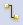
\includegraphics{Schematic_Wire.png} button to connect components
%%   with wires.

%% \item There are several PSpice power sources available. We will focus
%%   on four of the voltage sources available under \texttt{Place ->
%%     PSpice Component ... -> Source -> Voltage Sources}.
%%   \begin{itemize}
%%   \item \textbf{DC}\\
%%     The DC source produces constant voltage sources for bias point
%%     (DC) analysis. It has one parameter, \texttt{Vdc}, which sets the
%%     voltage of the source.
    
%%   \item \textbf{AC}\\
%%     The AC source produces sinusoidal wave forms for AC Sweep
%%     analysis. Its parameters are
%%     \begin{center}
%%       \begin{tabular}{ll}
%%         \texttt{Vac} & AC amplitude \\
%%         \texttt{Vdc} & DC offset
%%       \end{tabular}
%%     \end{center}
%%     (\textit{The frequency is controlled by the PSpice sweep
%%       analysis.})
%%   \item \textbf{Sine}\\
%%     The sine source produces sinusoidal wave forms for transient
%%     analysis. Its parameters are 
%%     \begin{center}
%%       \begin{tabular}{ll}
%%         \texttt{VOFF}  & Voltage offset \\
%%         \texttt{VAMPL} & Amplitude \\
%%         \texttt{FREQ}  & Frequency
%%       \end{tabular}
%%     \end{center}
%%     \textit{Ignore the \texttt{AC} parameter.}
    
%%   \item \textbf{Pulse}\\
%%     The pulse source can be used to produce periodic wave forms
%%     consisting of straight-line segments (square and triangle waves,
%%     e.g.) for transient analysis. The parameters of the pulse source
%%     are
%%     \begin{center}
%%       \begin{tabular}{ll}
%%         \texttt{V1}  & Low voltage \\
%%         \texttt{V2}  & High voltage \\
%%         \texttt{TR}  & Rise time from $V_1$ to $V_2$ \\
%%         \texttt{PW}  & Time at $V_2$ \\
%%         \texttt{TF}  & Fall time from $V_2$ to $V_1$ \\
%%         \texttt{PER} & Period \\
%%         \texttt{TD}  & Delay (shifts the entire waveform)
%%       \end{tabular}
%%     \end{center}
%%   \end{itemize}
  
%% \item The 
\includegraphics{Schematic_Cursor.png} button activates the
%%   cursor in the schematic. You can use the cursor to select
%%   components and wires, which you can then move or delete (with the
%%   \texttt{Delete} key). You can also right click on a component to
%%   change its orientation by selecting \texttt{Rotate},
%%   \texttt{Mirror Horizontally}, \texttt{Mirror Vertically}, or
%%   \texttt{Mirror Both}.

%% \item Models of many components beyond the generic PSpice components
%%   are available via the part search panel opened by \texttt{Place ->
%%     Part ...}. The part libraries are not loaded by default. To add a
%%   library, click on the 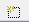
\includegraphics{OrCAD_AddLib.png} button, and
%%   select from the list. If you do not see a list of libraries
%%   (\texttt{.olb} files), use the file browser to navigate to:
%%   \begin{quote}
%%     \verb+C:\Cadence\SPB_17.2\tools\capture\library\pspice+
%%   \end{quote}
%% \end{itemize}

%% \subsection{Simulation Profile}

%% Once you have completed the schematic of the circuit you want to
%% simulate, create a simulation profile:

%% \begin{enumerate}
%% \item Click on \texttt{PSpice -> New Simulation Profile} or use the
%%   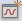
\includegraphics{OrCAD_NewSimProf.png} button in the tool bar.

%% \item Name the profile.

%% \item Choose an analysis type --- either \texttt{Bias Point} to
%%   investigate steady-state behavior, \texttt{Time Domain
%%   (Transient)} to investigate time-dependent behavior,
%%   or \texttt{AC Sweep/Noise} to investigate the frequency response
%%   of the circuit.
%%   \begin{itemize}
%%   \item For \texttt{Time Domain (Transient)}, set the \texttt{Run
%%     To Time} value to the length of time over which you would like to
%%     simulate the behavior of your circuit. Make sure you are using one
%%     of the transient voltage sources (\texttt{Sine} or
%%     \texttt{Pulse}). 
    
%%   \item For \texttt{AC Sweep/Noise} analysis, fill in the \texttt{AC
%%     Sweep Type} panel (\texttt{Start Frequency}, \texttt{End
%%     Frequency}, and \texttt{Points/Decade}). You will usually want a
%%     logarithmic sweep. Make sure you are using an \texttt{AC} voltage
%%     source. 
%%   \end{itemize}

%%   \item If you need to go back and edit a profile, use \texttt{PSpice
%%     -> Edit Simulation Profile} or the
%%     
\includegraphics{OrCAD_EditSimProf.png} button in the tool bar.
%% \end{enumerate}

%% Then, in the schematic window, click on the 
%% 
\includegraphics{OrCAD_RunSim.png} button in the tool bar to run the
%% simulation. 

%% \subsection{Viewing Steady-State Results}

%% In DC circuits, steady-state behavior is constant, and plotting the
%% time dependence is not helpful. Instead, after running the simulation,
%% click on the 
\includegraphics{OrCAD_ShowV.png} and
%% 
\includegraphics{OrCAD_ShowI.png} buttons in the tool bar in the 
%% schematic window to display voltages and currents. The
%% 
\includegraphics{OrCAD_ShowI.png} button displays power
%% dissipated/stored/delivered for each device.

%% \textit{Note: There is a known bug that prevents the voltage and
%%   currents displayed in the schematic from updating after you modify
%%   the circuit. The work-around is to close the schematic tab (usually
%%   titled \texttt{PAGE1}) and reopen it by double-clicking on the
%%   schematic under \texttt{Design Resources -> <Project Name>.dsn ->
%%     SCHEMATIC1 -> PAGE1} in the project tab.}

%% \subsection{Plots}

%% When you run a simulation, a separate \texttt{PSpice AD Lite} window
%% will open in the background. This window will show a plot with time on
%% the horizontal axis for a transient analysis or frequency on the
%% horizontal axis for a sweep analysis. In \texttt{PSpice AD Lite}, a
%% graph of a quantity is called a \textbf{trace}, in reference to
%% oscilloscope traces. Multiple traces can be displayed on the plot.

%% \subsubsection*{Markers and Traces}

%% To automatically plot voltages or currents, add markers to your
%% schematic using the marker buttons in the tool bar of the schematic  
%% window prior to running the simulation.
%% \begin{itemize}
%% \item[
\includegraphics{OrCAD_VMarker.png}] A voltage marker should be
%%   placed on a wire between devices. It measures voltage relative
%%   to ground.  

%% \item[
\includegraphics{OrCAD_DiffVMarker.png}] Voltage differential
%%   markers are placed in pairs and measure the voltage between two points. 

%% \item[
\includegraphics{OrCAD_IMarker.png}] A current marker must be
%%   placed at junction between a device and a single wire. It
%%   measures the current flowing through that point.

%% \item[
\includegraphics{OrCAD_WMarker.png}] Power markers must be
%%   placed on a devices. It measured the power supplied / dissipated /
%%   stored by a device.
%% \end{itemize}
%% Markers are associated with analysis profiles rather than with the
%% schematic itself, so you can specify different markers for different
%% analysis profiles.

%% Traces can also be added ``by hand'' using
%% \texttt{Trace -> Add Trace...} or the
%% 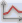
\includegraphics{PSpiceAD_AddTrace.png} button. To display traces with
%% different units (voltage and power, e.g.) on the same plot, use
%% \texttt{Plot -> Add Y Axis}, and select each axis in turn, adding a
%% trace(s) to each one.

%% \subsubsection*{Trace ``Measurements''}

%% The plot panel in \texttt{PSpice AD Lite} is designed to function
%% somewhat like a digital oscilloscope. The
%% 
\includegraphics{PSpiceAD_Cursor.png} button in the  tool bar enables
%% a pair of cursors in the plot. Left-clicking places cursor 1, and
%% right-clicking places cursor 2. Cursor positions and differences are
%% displayed in the cursor window, which is displayed when the cursor is
%% activated. If the plot panel contains more than one trace, each cursor
%% is tied to a particular trace. Left-click on a trace label to tie
%% cursor 1 to the corresponding trace, and right-click on a trace label
%% to tie cursor 2 to the corresponding trace.

%% A collection of automated measurements (period, zero crossing time,
%% high-pass and low pass cutoffs, band width, e.g.) can be defined using
%% the 
\includegraphics{PSpiceAD_DefineMeasurement.png} button. The 
%% 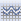
\includegraphics{PSpiceAD_ToggleMeasurement.png} button toggles the
%% display of the measurement results.

%% \subsubsection*{Exporting Trace Data}

%% You can right-click on a trace and choose \texttt{Copy to Clipboard}
%% to paste the corresponding data directly into a spreadsheet or text
%% file. \texttt{File -> Export -> Text} or
%% \texttt{File -> Export -> Comma Separated File} can also be used to
%% save all trace data to a text file that can be read into other
%% analysis programs.

\end{document}
